\documentclass{article}[12pt]
\usepackage{physics}
\usepackage{setspace}
\usepackage{amsmath}
\usepackage{mathrsfs}
\usepackage{amssymb}
\usepackage{feynmp-auto}
\usepackage{tgtermes}
\usepackage{graphicx}
\usepackage{booktabs}
\usepackage{array}
\usepackage{caption}
\usepackage{listings}
\usepackage{xcolor}
\usepackage{helvet}
\usepackage{float}
\definecolor{codegreen}{rgb}{0,0.6,0}
\definecolor{codegray}{rgb}{0.5,0.5,0.5}
\definecolor{codepurple}{rgb}{0.58,0,0.82}
\definecolor{backcolour}{rgb}{0.95,0.95,0.92}
\definecolor{lightgray}{rgb}{0.95,0.95,0.95}

\lstdefinestyle{mystyle}{
    backgroundcolor=\color{lightgray},   
    commentstyle=\color{codegreen},
    keywordstyle=\color{magenta},
    numberstyle=\tiny\color{codegray},
    stringstyle=\color{codepurple},
    basicstyle=\fontfamily{pcr}\selectfont\footnotesize,
    breakatwhitespace=false,         
    breaklines=true,                 
    captionpos=b,                    
    keepspaces=true,                 
    numbers=left,                    
    numbersep=5pt,                  
    showspaces=false,                
    showstringspaces=false,
    showtabs=false,                  
    tabsize=2
}
\setcounter{page}{28}
\setcounter{figure}{13}
\setcounter{table}{2}
\setcounter{section}{3}
\lstset{style=mystyle}
\captionsetup{font=footnotesize}
\newcommand{\RN}[1]{%s
  \textup{\uppercase\expandafter{\romannumeral#1}}%
}
\usepackage{geometry}
\geometry{
 a4paper,
 left=25.4mm,
 right=25.4mm,
 top=30mm,
 bottom=25.4mm
 }
\begin{document}
\section{Result}
\begin{spacing}{1.3}
\subsection{Benchmark Setup and Simulation Environment}
\subsubsection*{Benchmark: Exact diagonalization in single mode}
To compare with the result from exact diagonalization (ED), we set the condition when the bath has only a single mode. 
The result shows that the approximation method could be reliable in high temperatures ($\beta = 1$). Throughout the result analysis, we use $k_b$ as unit value 1.
\begin{figure}[htbp]
  \centerline{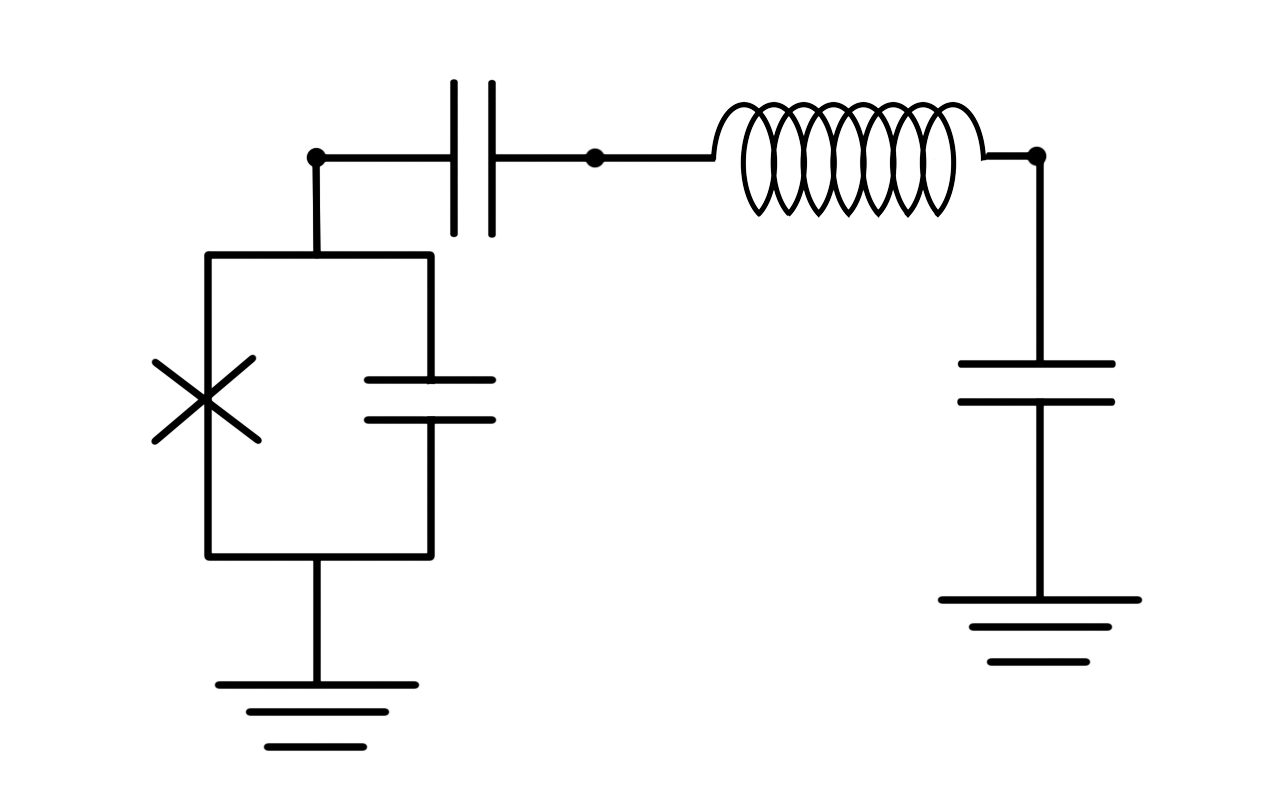
\includegraphics[width=7cm]{TexFigure/4/4_1_00_Singlebath.png}}
  \caption{Brief circuit scheme for single bath condition. The crossing symbol  refers to the junction structure.}
\end{figure}
\begin{figure}[htbp]
  \centerline{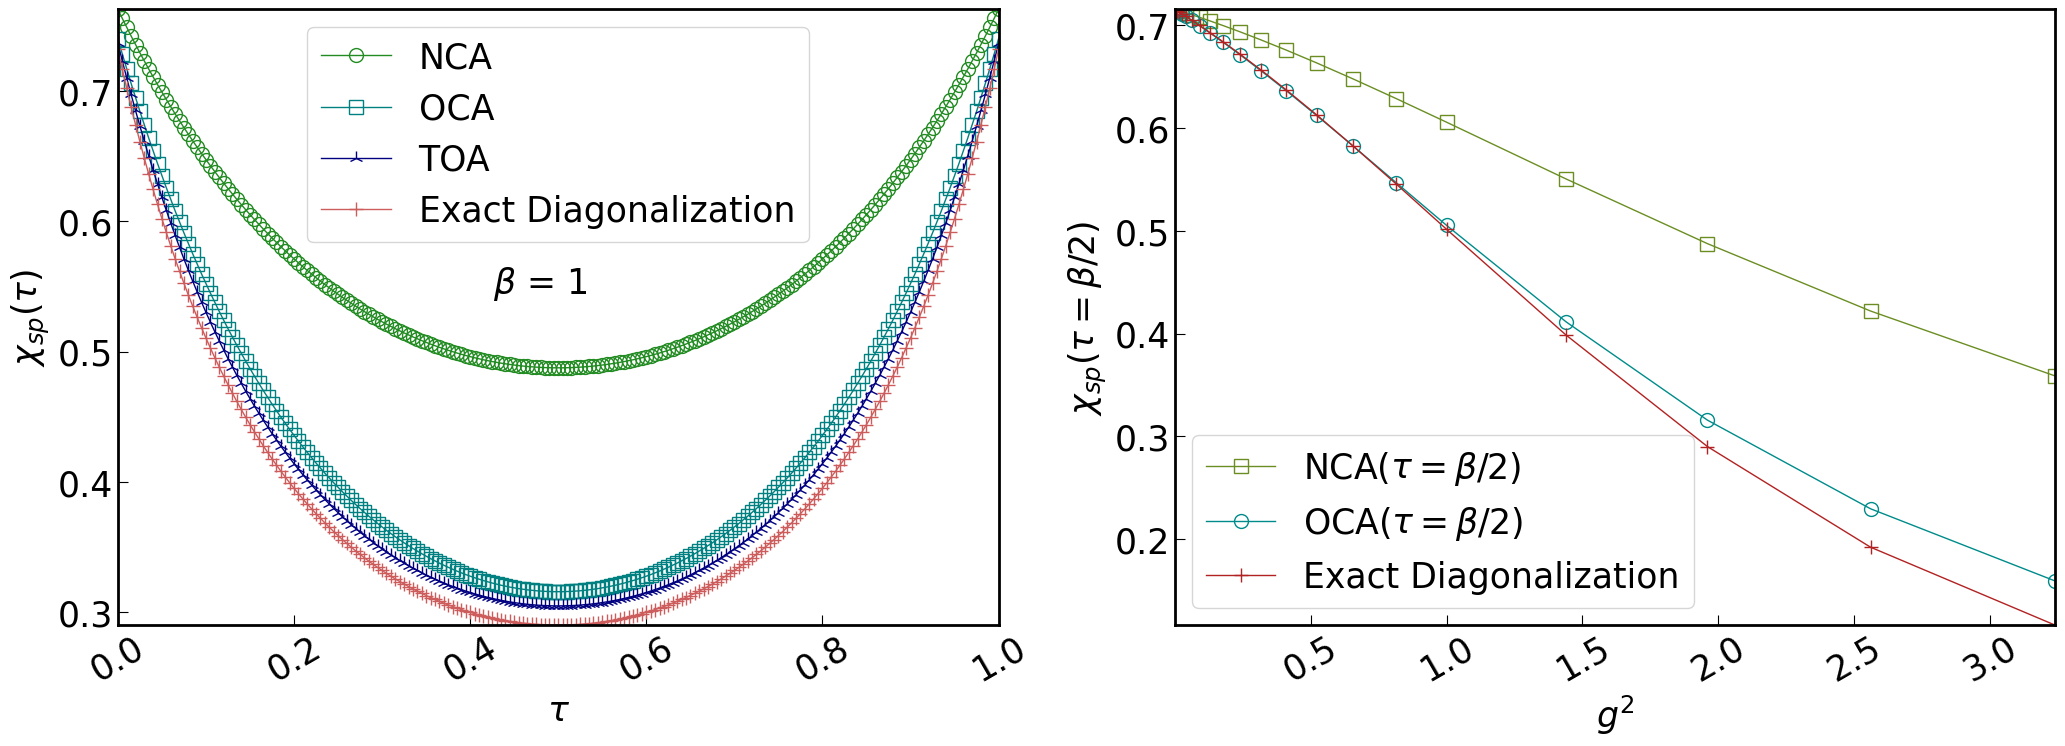
\includegraphics[width=13cm]{TexFigure/4/4_1_01_Single.png}}
  \caption{Result for single bath benchmark. In the left figure, the overall condition for g (coupling strength between system and bath) is 1. The right figure shows the result in the OCA approaches to the exact results.}
\end{figure}\pagebreak
\subsubsection*{Benchmark: Multi-mode case}
To investigate the convergence of the diagrammatic approximation method in a general bosonic reservoir condition, 
we calculated the order parameter and the correlation function using the NCA, OCA, and TOA. 
The results showed no significant difference between the OCA and TOA calculations, confirming that the OCA is a sufficiently convergent method.
\begin{figure}[H]
  \centerline{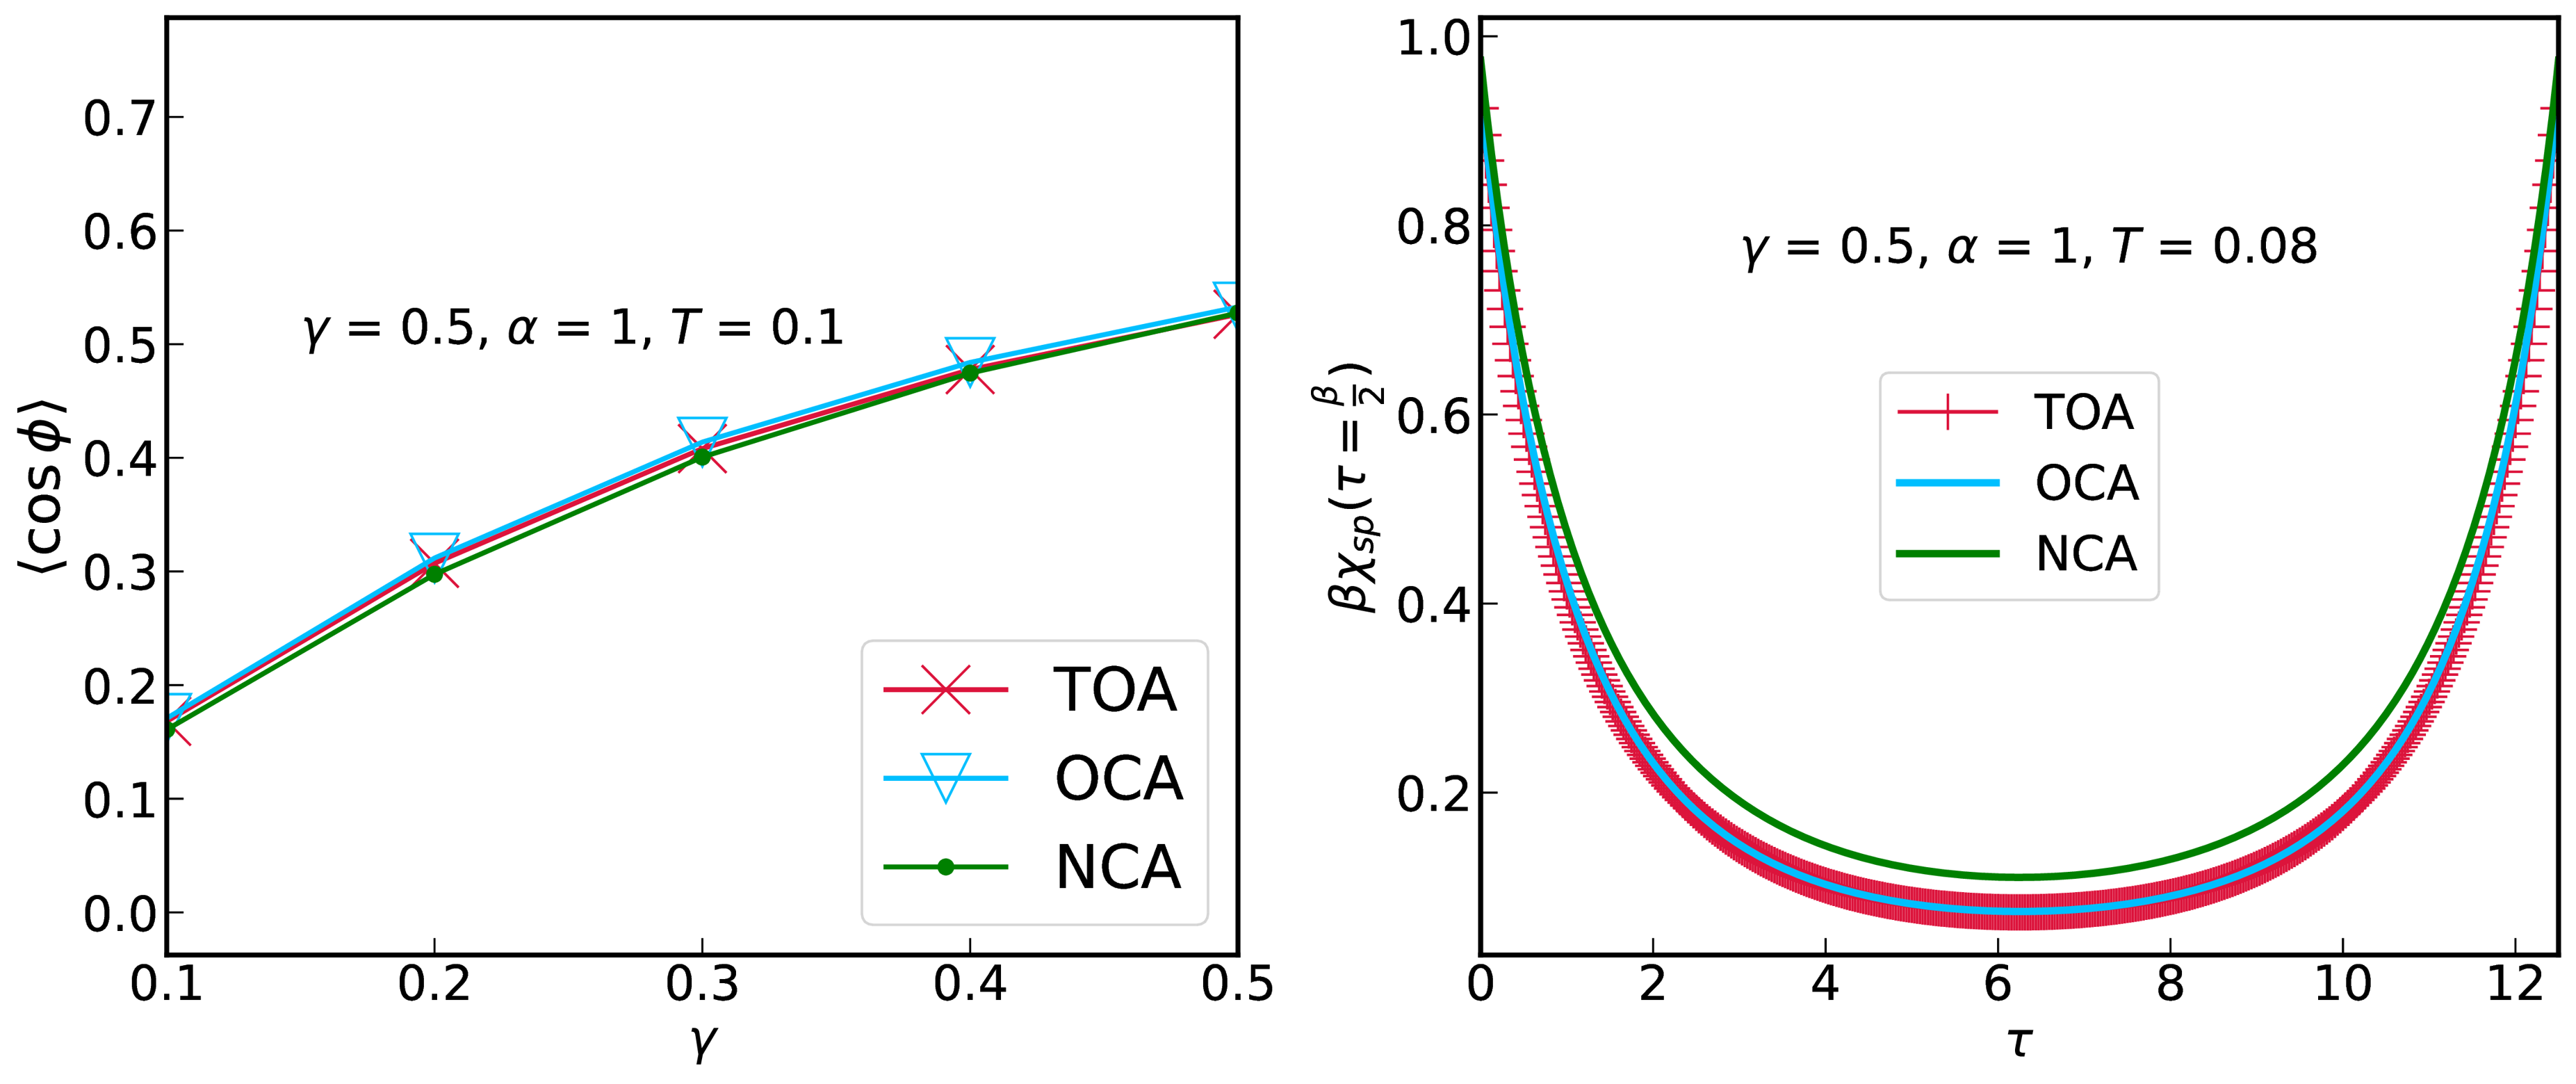
\includegraphics[width=13cm]{TexFigure/4/4_1_02_Multi.png}}
  \caption{Results of the order parameter and correlation function calculated under each approximation method. 
  The overall parameter conditions are $\alpha$=1, $\gamma$=1, with the left figure showing the result in a temperature interval between 0.08 and 0.1; the right figure is for the temperature condition of 0.08. It can be observed that the calculation results of OCA and TOA are converged. 
  The size of the $\tau$ grid used for the calculation is 701.}
 \end{figure}
\subsubsection*{Benchmark: $\alpha$ = 0 condition}
To check for the integration code, we compared the order parameter calculated using approximation methods for the case of α=0 
with the order parameter calculated using the state density matrix of the Josephson junction system. 
The results showed that the two cases were entirely consistent.
\begin{figure}[H]
  \centerline{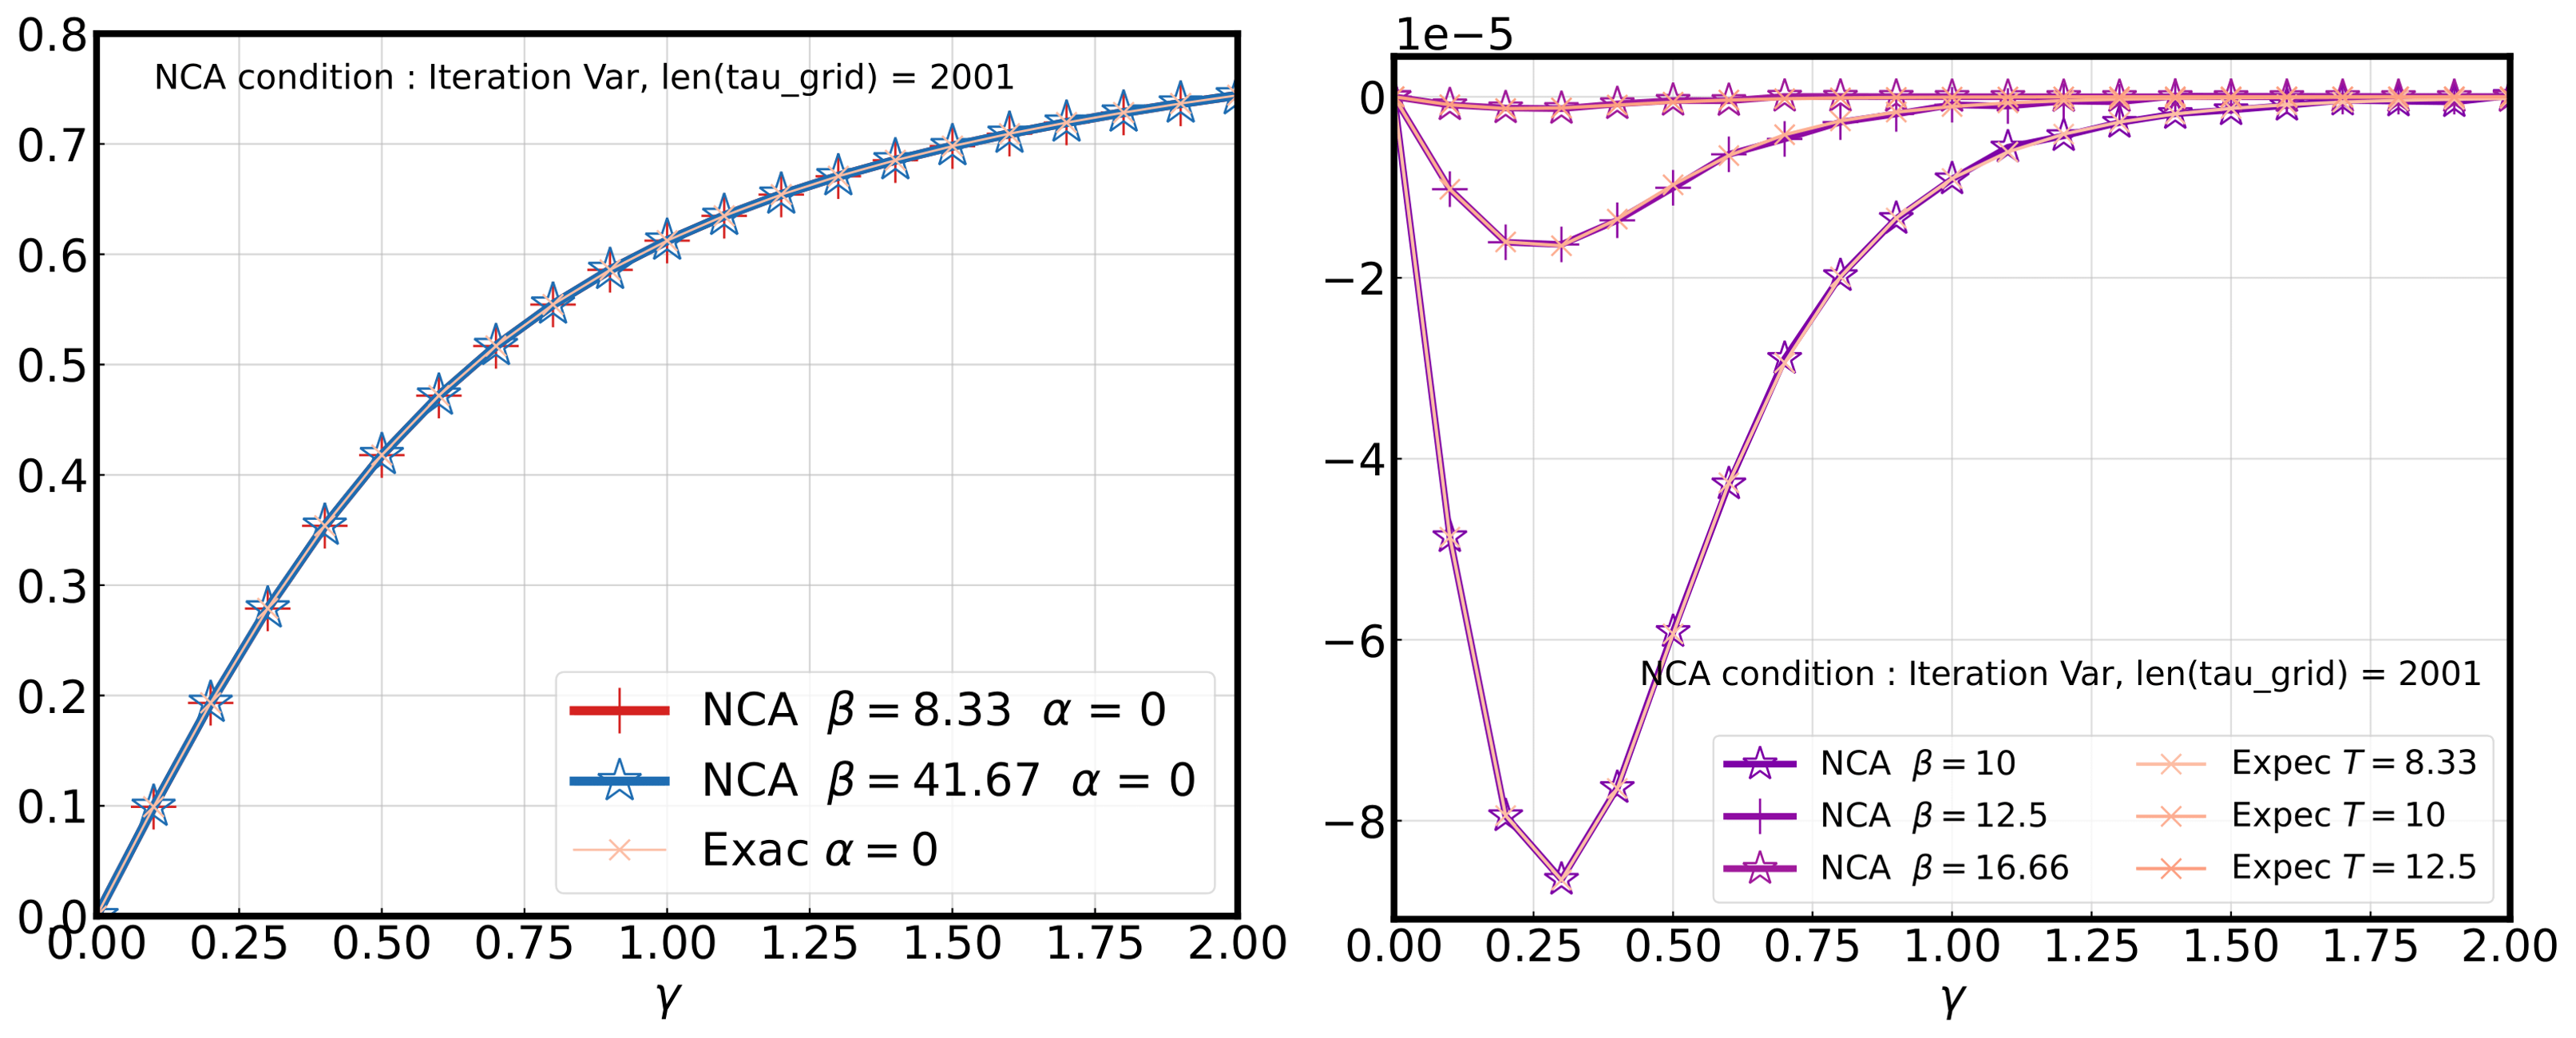
\includegraphics[width=13cm]{TexFigure/4/4_1_03_zero.png}}
  \caption{In the case of $\alpha = 0$, order parameter calculation using the approximation method should be consistent with using $H_{loc}$.
  The comparison confirmed that the two cases show consistency. The left figure shows the calculation of the order parameter, 
  and the right figure shows the difference in the order parameter for consecutive $\beta$ values
  in the intervals [8.33, 10], [10, 12.5], and [12.5, 16.6].}
 \end{figure}
\pagebreak
\subsubsection*{Simulation condition: Saturation test}
The factors influencing the accuracy of the approximation method are the number of integration iterations and the size of the τ grid.
We investigated the convergence behavior of the calculation results for changing the order parameter. 
We confirmed that the results converge for the case of a tau grid size of 1800 to 2000. 
\begin{table}[htbp]
  \centering
  \renewcommand{\arraystretch}{1.2}  % 행 간격 조정
  \begin{tabular}{@{}ccc@{}}
  \toprule
  \textbf{Number} & \textbf{Interval} & \textbf{Gridsize}\\ 
  \midrule
  $\tau$ grid & [0,$\beta$] & 2000 \\
  k grid & [0,K = 30000] & 30000 \\
  \bottomrule
  \end{tabular}
  \caption{Grid condition used for calculation.}
  \end{table}
\begin{figure}[htbp]
  \centerline{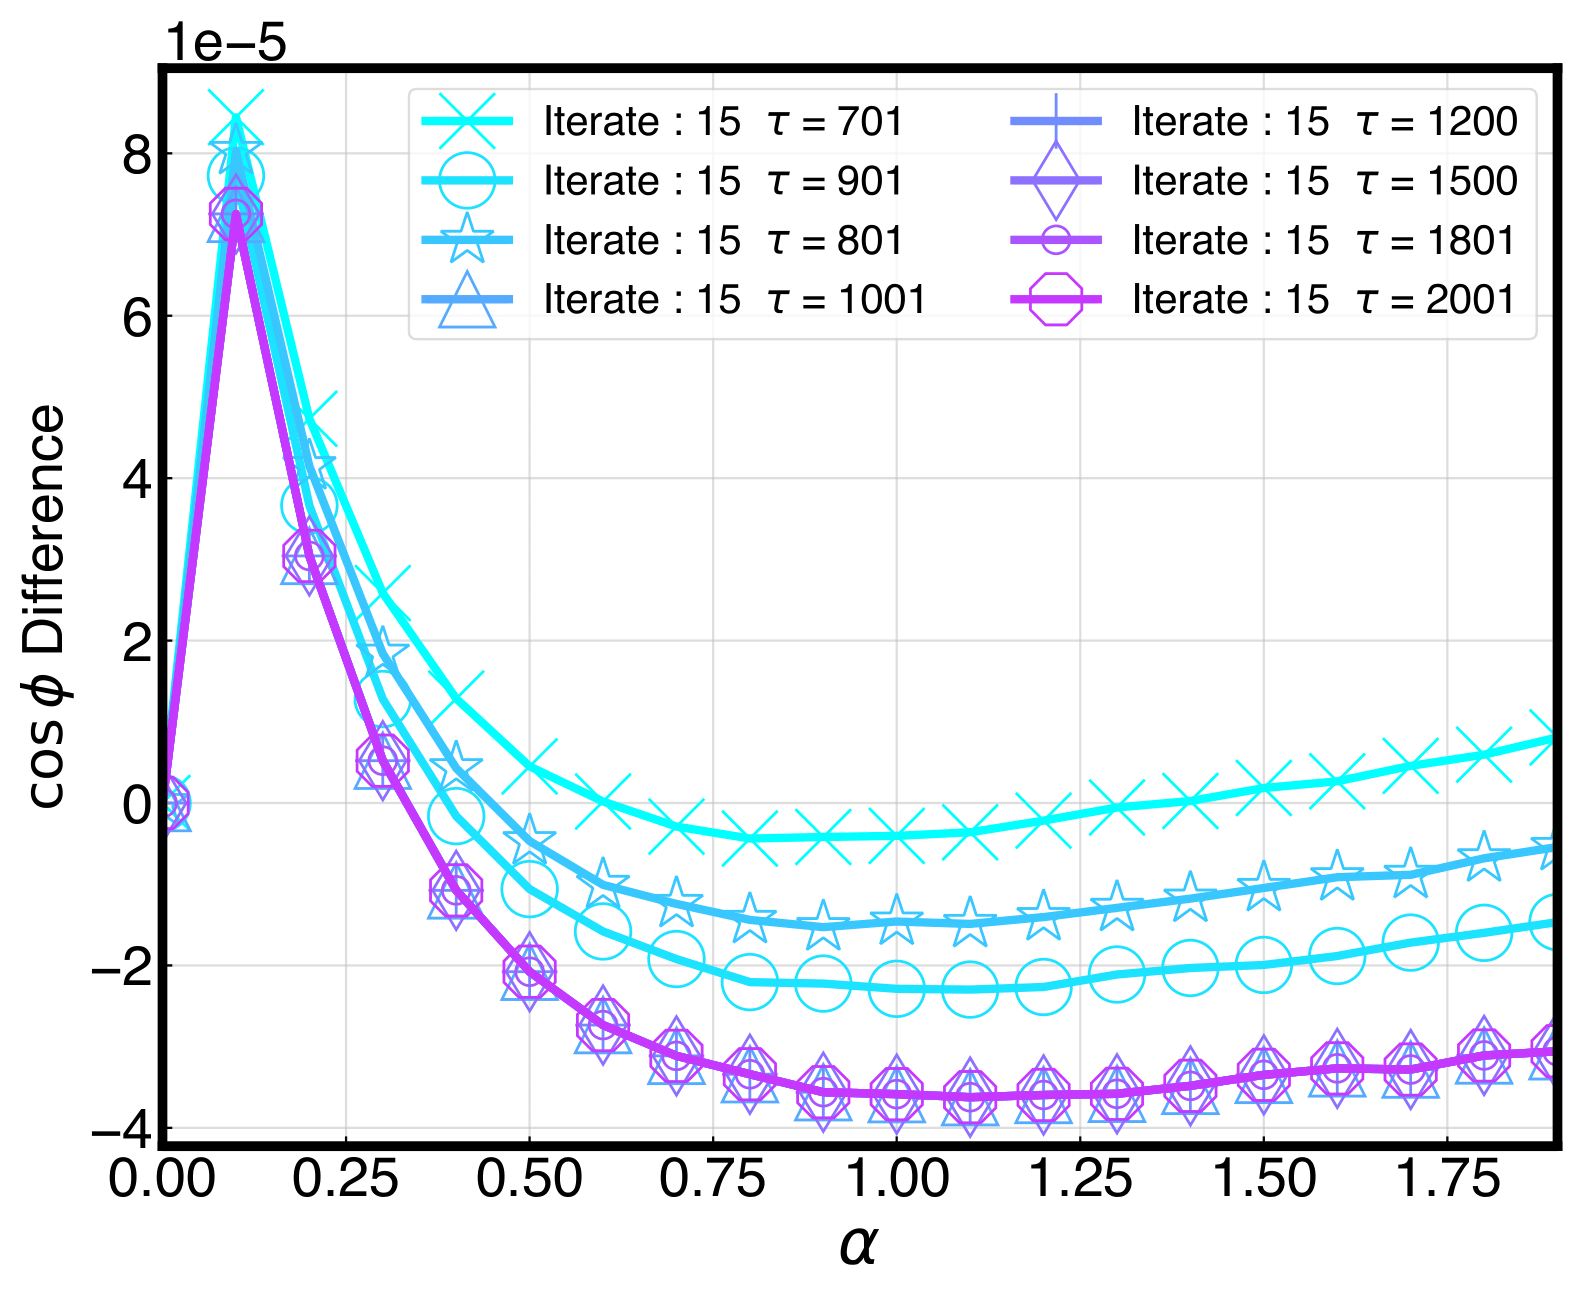
\includegraphics[width=7.5cm]{TexFigure/4/4_2_01_saturation.png}}
  \caption{Saturation test in different time grid size. The temperature condition is $\beta = 41.67$}
\end{figure}
\pagebreak
\subsubsection*{Simulation condition: Size dependence}
Since the resistively shunted Josephson junction circuit corresponds to a model that the physical system has coupled to the waveguide structure,
there was a breakdown of the rotating wave approximation of the two-level system as the coupling strength between the RC resonator circuit 
and the Josephson junction increases[15]. The test condition is $\gamma =2$, $\alpha = 1.5$ with calculating correlation function. 
The benchmark result shows that adopting a 2-level truncated condition is reliable since the difference between the two sizes is ignorable.
\begin{figure}[H]
  \centerline{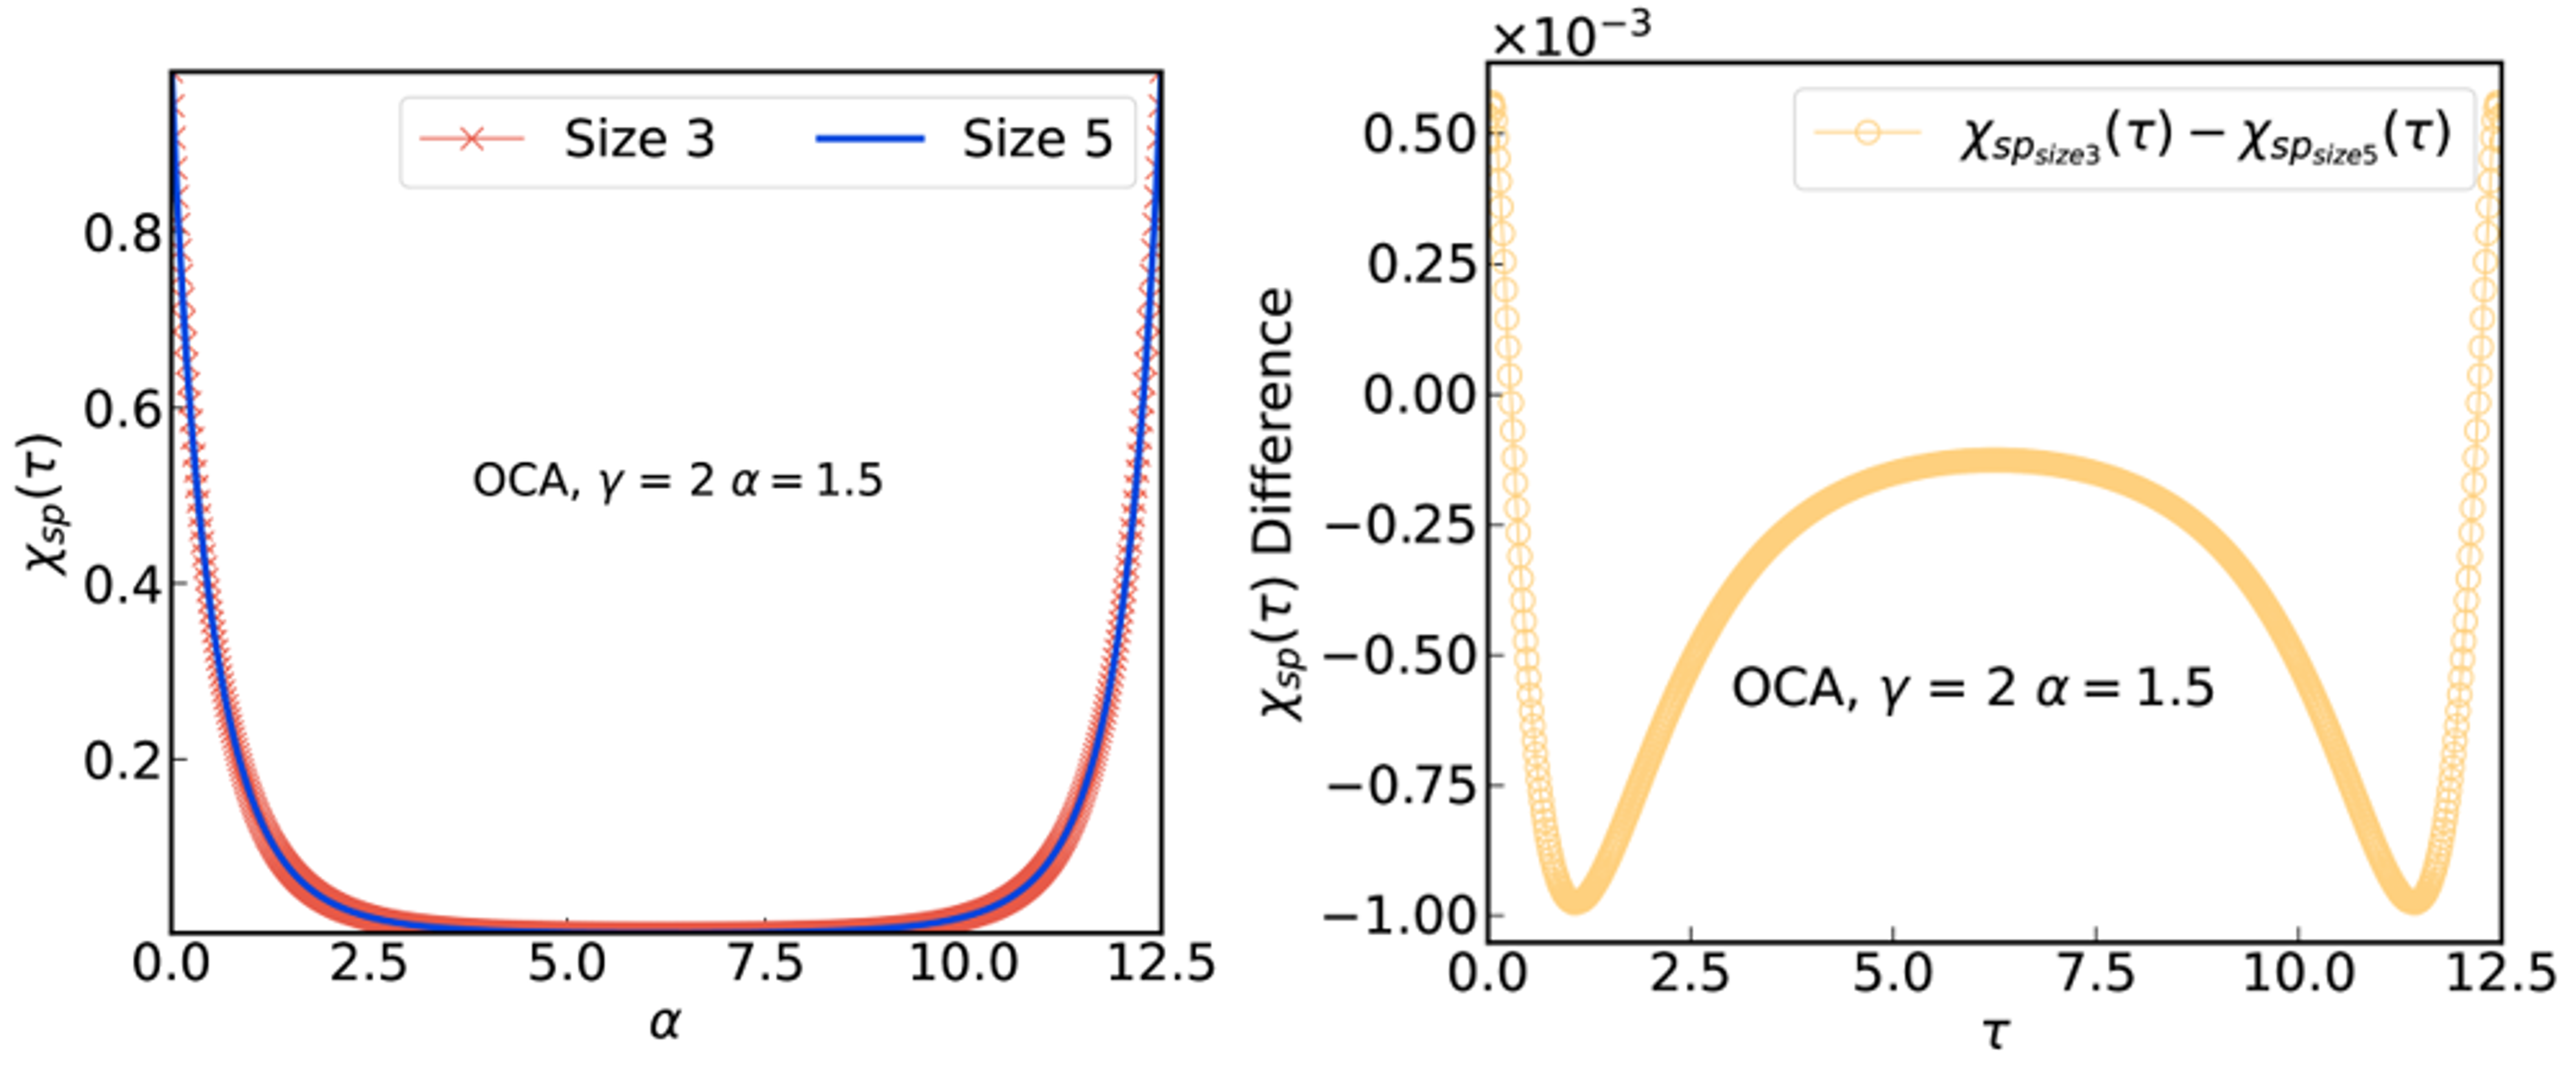
\includegraphics[width=13cm]{TexFigure/4/4_2_02_sizediff.png}}
  \caption{Comparision with $\chi_{sp}(\tau)$ size3 and size5. The size of the $\tau$ grid used for the calculation is 701.}
\end{figure}
\subsection{Orderparmeter evaluation}
Regarding the previous study, which reported that the transition occurs at $\alpha = 1$, we set the range of parameters around $\alpha = 1$ and $\gamma = 1$.
We set the range of variables used in the simulation as Table 4.
\begin{table}[htbp]
  \centering
  \renewcommand{\arraystretch}{1.2}  % 행 간격 조정
  \begin{tabular}{@{}cccc@{}}
  \toprule
  \textbf{Variables} & \textbf{Min} & \textbf{Max}  & \textbf{Interval}\\ 
  \midrule
  $\gamma$ & 0 & 2 & 0.1 \\
  $\alpha$ & 0 & 2 & 0.01 \\
  $\beta$ & 7.14 & 62.5 &  \\
  Temperature & 0.016 & 0.14 & 0.02 (until 0.04) \\
  \bottomrule
  \end{tabular}
  \caption{Parameter interval used for calculation.}
  \end{table}
\subsubsection*{Temperature independent result}
First, we calculated the expectation value of the order parameter $\hat{\cos\phi}$ 
over the given range of $\gamma$. The results showed that the Josephson junction exhibited superconducting behavior 
as its nonlinearity increased at all temperatures. Subsequently, we compared the diagonal elements of the product 
of the operator $\hat{\cos\phi}$ and the operator $\hat{H_{\text{loc}}}$, both expressed in matrix form, 
for different degrees of coupling with the external environment. We expected the probability of the system 
being in the ground state to be the highest without considering the $\alpha$ value. From the result, 
it can be deduced that the system shows the superconductor state, consistent with the observed
result from the expectation value of the order parameter.
\pagebreak
\begin{figure}[H]
  \vfill
  \centerline{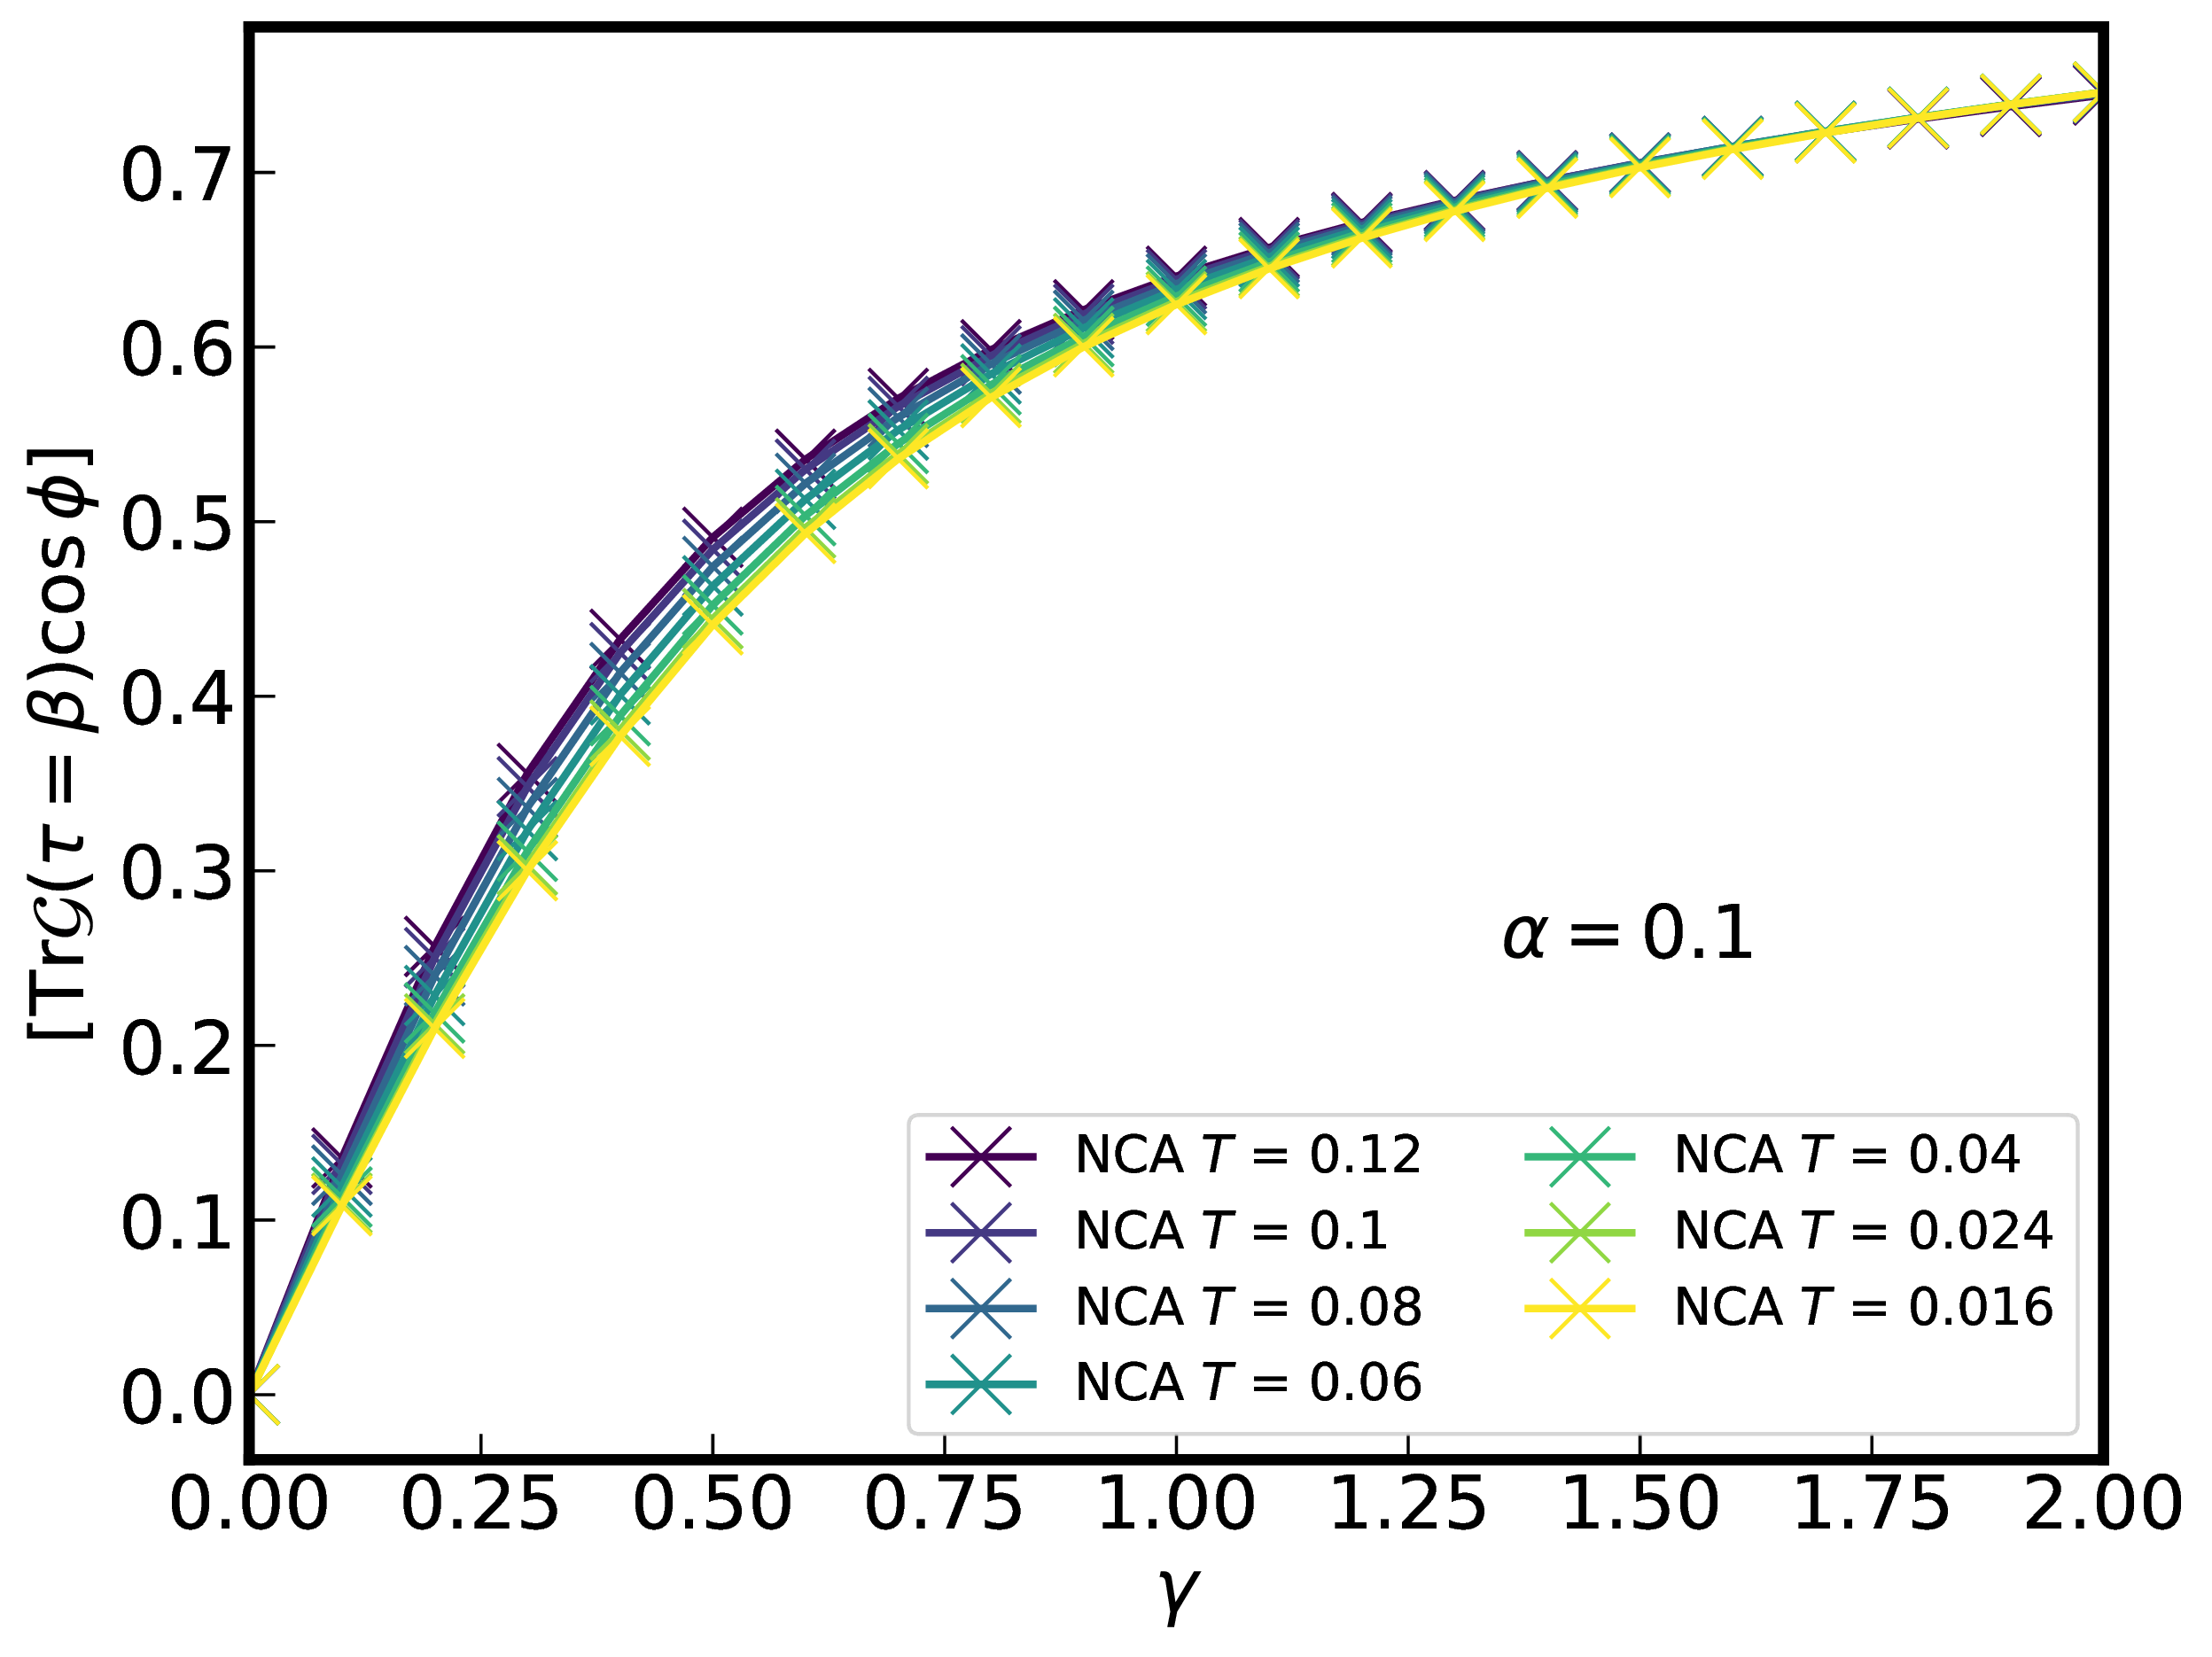
\includegraphics[width=8cm]{TexFigure/4/4_3_01_Expec_alp_0.1.png}}
  \caption{Calculation of the expectation value of the order parameter for the case of $\alpha$=0.1.}
  \label{fig:Order1}
  \vfill
\end{figure}
\begin{figure}[H]
  \vfill
  \centerline{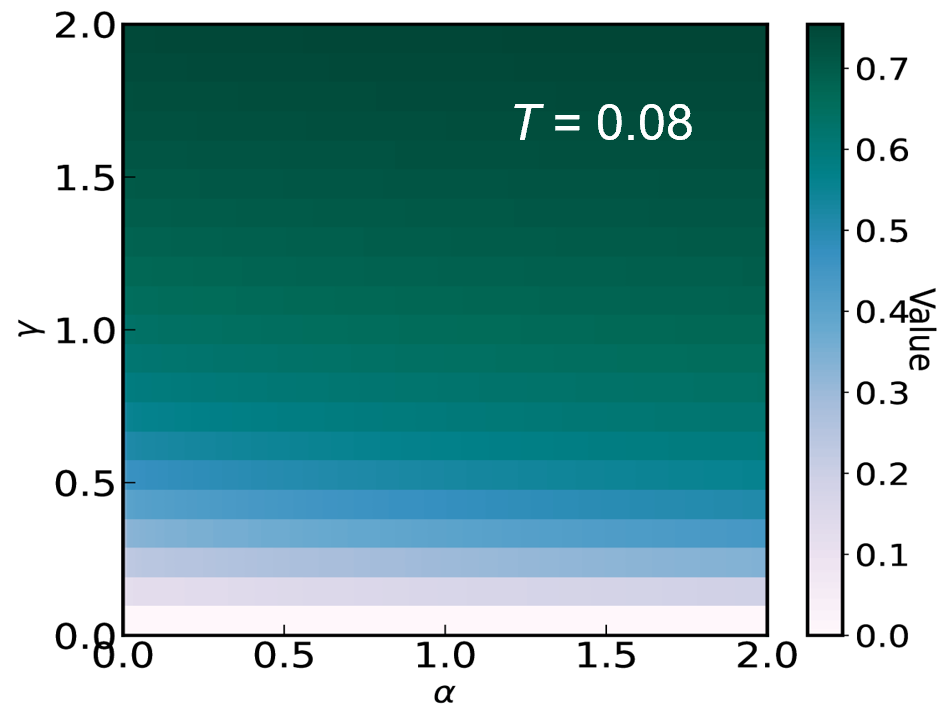
\includegraphics[width=8cm]{TexFigure/4/4_3_02_Temp.png}}
  \caption{Colored plot for the expectation value of order parameter. The simulation was performed in NCA. The temperature condition is T = 0.08
  The difference in phase on each side of the junction decreases as the color goes deeper, corresponds to superconductivity.}
  \vfill
\end{figure}
\pagebreak
\begin{figure}[htbp]
  \centerline{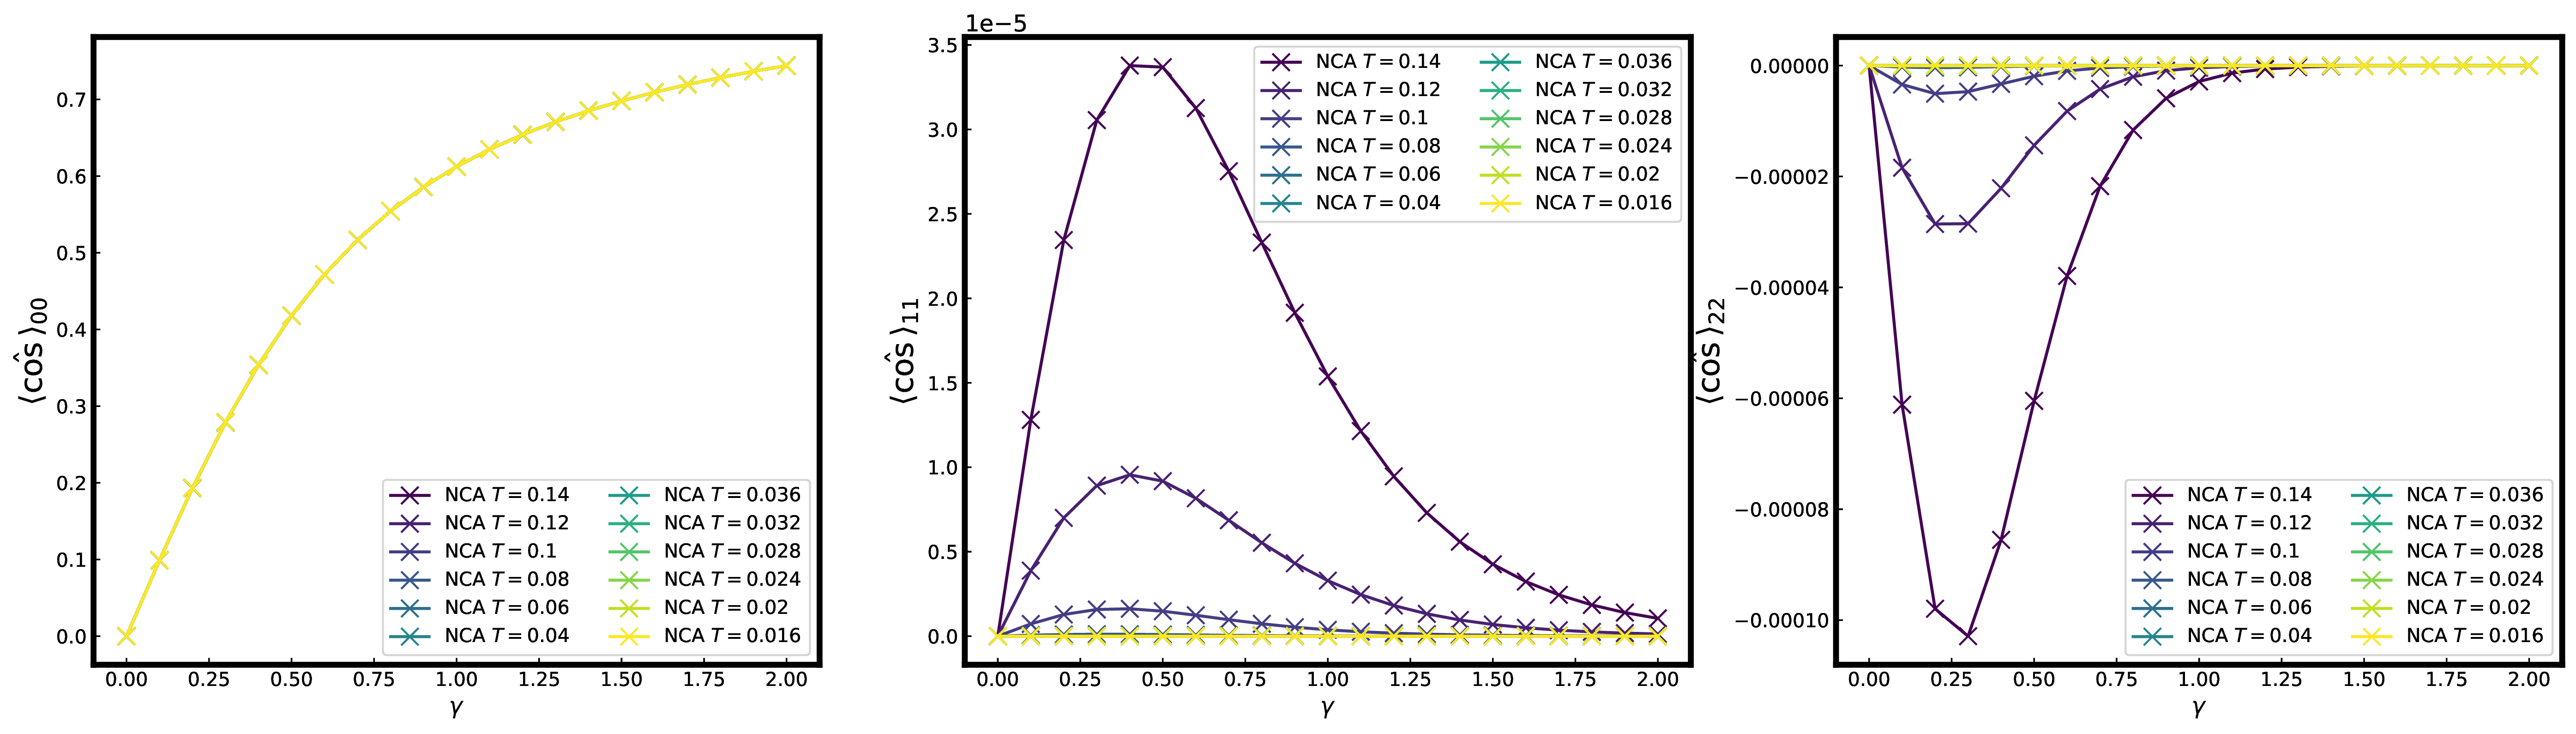
\includegraphics[width=15cm]{TexFigure/4/4_3_03_Matele_Ns3_alp0.png}}
  \centerline{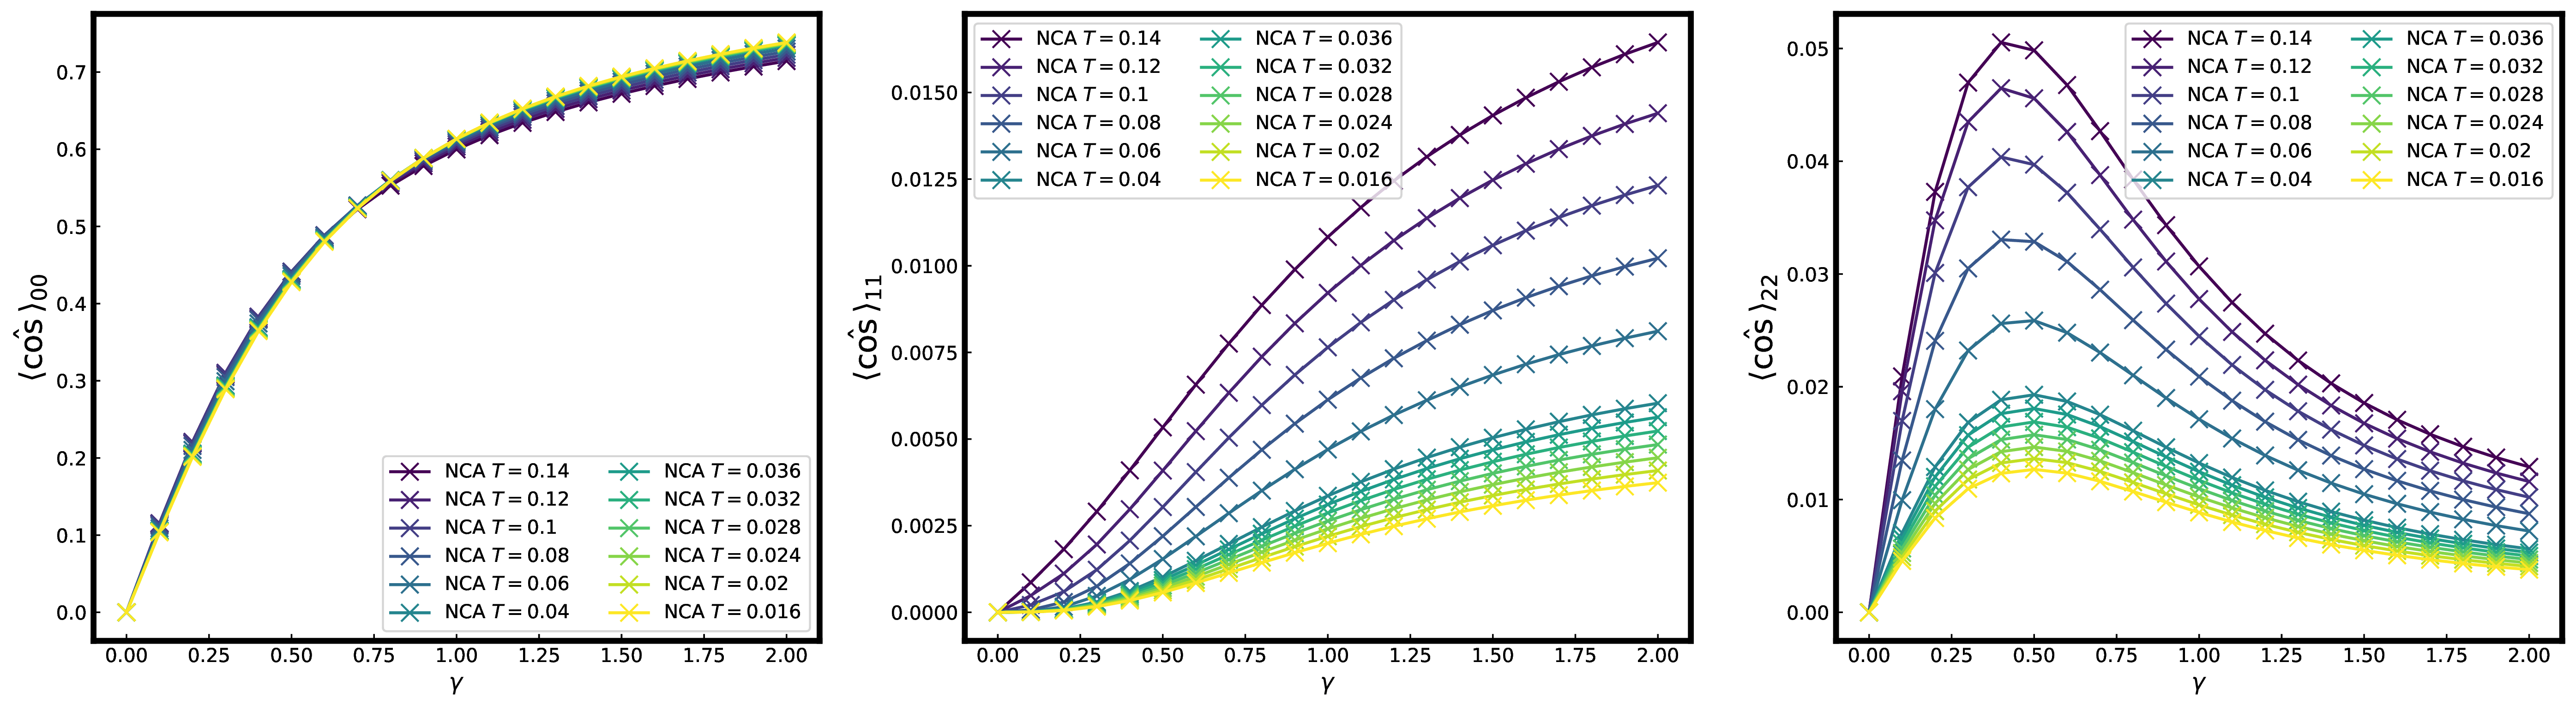
\includegraphics[width=15cm]{TexFigure/4/4_3_04_Matele_Ns3_alp0_1.png}}
  \centerline{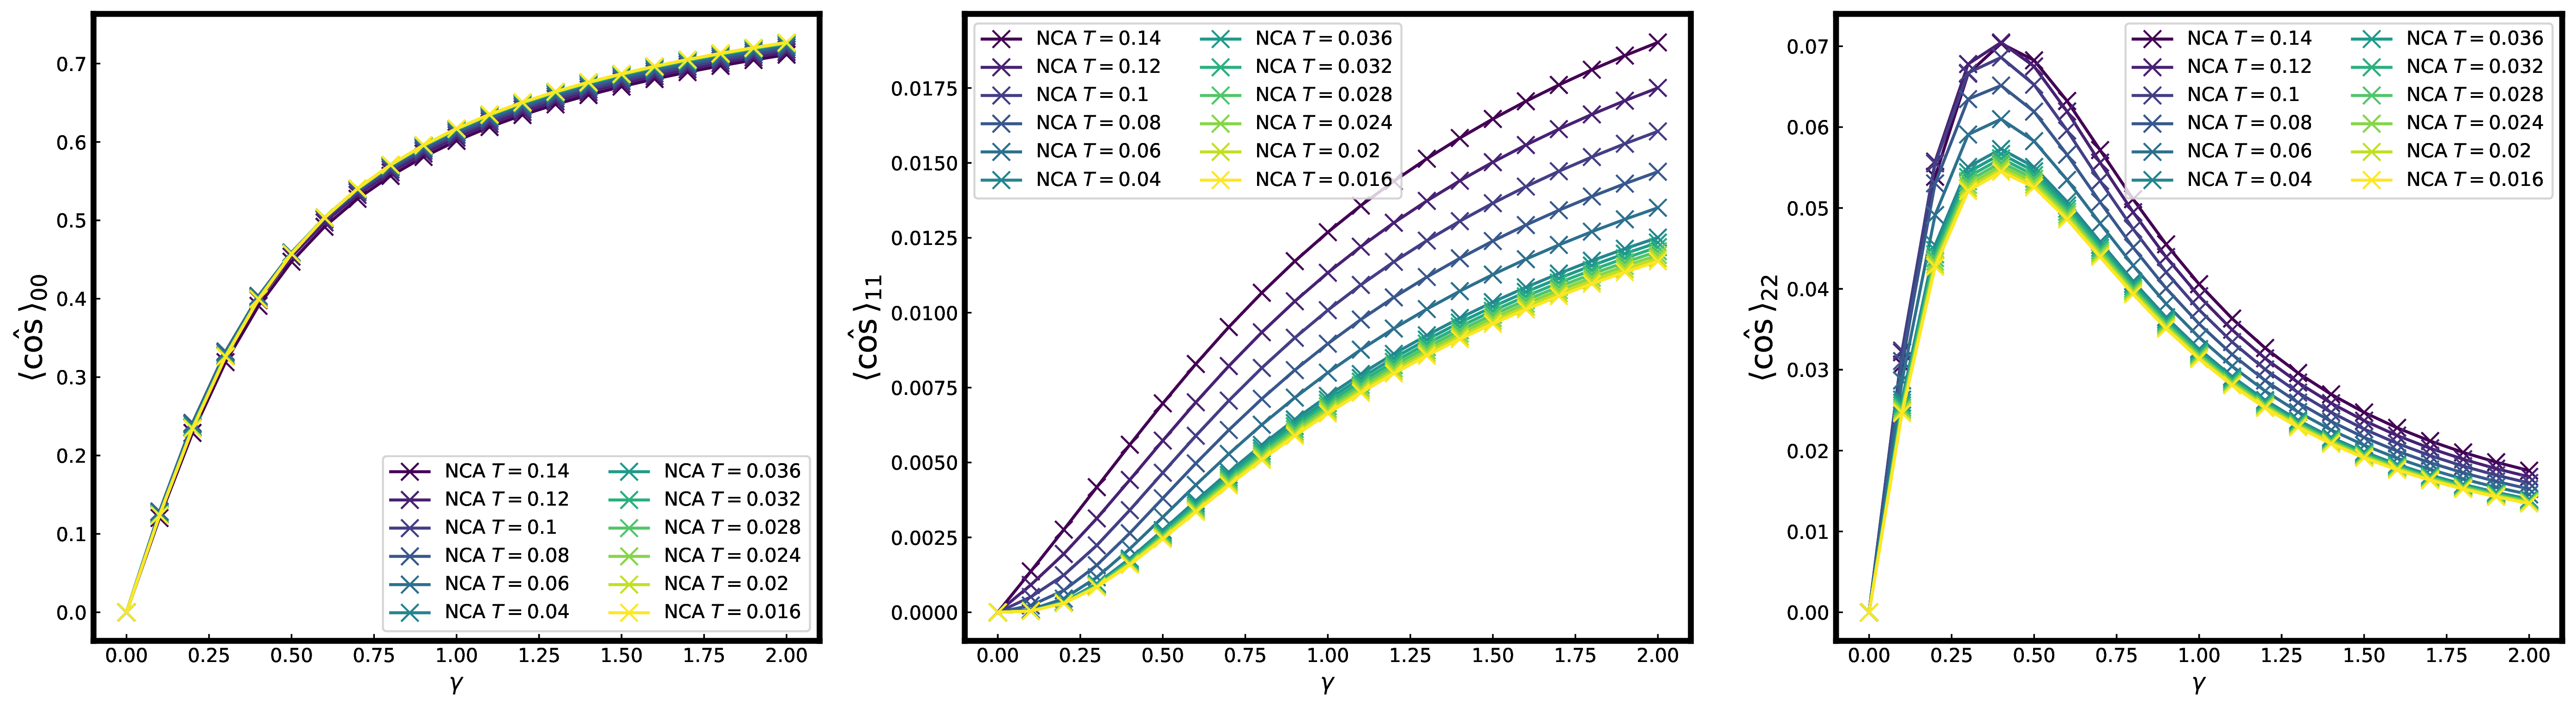
\includegraphics[width=15cm]{TexFigure/4/4_3_05_Matele_Ns3_alp1.png}}
  \caption{Plotted results of the diagonal elements of the product of the $\hat{\cos\phi}$ operator and the  
  $e^{H_{loc}}$ operator for different $\alpha$ values. From top to bottom, the results are for $\alpha$ 
  values of 0, 0.01, and 0.1, respectively. The first diagonal element is proportional to the probability of 
  the system being in the ground state, which shows having the largest value among the diagonal elements 
  for all $\alpha $and $\gamma$ values. This confirms that the system tends to superconductivity regardless of 
  adjusting parameters.}
  \end{figure}
\pagebreak
\subsubsection*{Temperature dependent transition}
To determine the criticality of the system's phase concerning temperature, 
a new order parameter $\nu(T,\alpha,\gamma)$ was introduced, its change concerning temperature was defined as follows:
\begin{flalign}
  \begin{split}
\frac{\partial \nu}{\partial T} \approx \frac{ \langle\hat{\cos \phi}\rangle|_{T_i} - \langle\hat{\cos \phi}\rangle|_{T_{i+1}}}{\Delta T} \quad , \quad \Delta T = |T_{i}-T_{i+1}|
\end{split}
\end{flalign}
Following the equation above, we observed the changes in the order parameter while varying the temperature. As the temperature decreases, the tangent of the order parameter changes from a high to a low slope. This allows us to predict the temperature-dependent behavior of the system under investigation. The prediction of the system's phase change according to $\frac{\partial \nu}{\partial T}$ is follows:
\begin{flalign}
\begin{split}
\begin{cases}\frac{\partial \nu}{\partial T} > 0 \quad : \quad \text{Insulating} \\ \frac{\partial \nu}{\partial T} < 0 \quad : \quad \text{Superconducting}\\
\frac{\partial \nu}{\partial T} =0 \quad : \quad \text{crossover point}\end{cases}
\end{split}
\end{flalign}
When the simulation results were plotted on the $\alpha − \gamma$ plane, following three features were observed :\\
\indent 1. $\alpha$=0 (no interaction with the external reservoir), the system exhibits superconducting properties.\\
\indent 2. Crossover points on the $\alpha - \gamma$ plane for each consecutive temperature range, the left side of the crossover line predicted as insulating properties and superconducting properties for the right side.\\
\indent 3. As the temperature decreases, the range exhibiting insulating properties widens for a given $\alpha$ interval.\\
\begin{figure}[H]
  \centerline{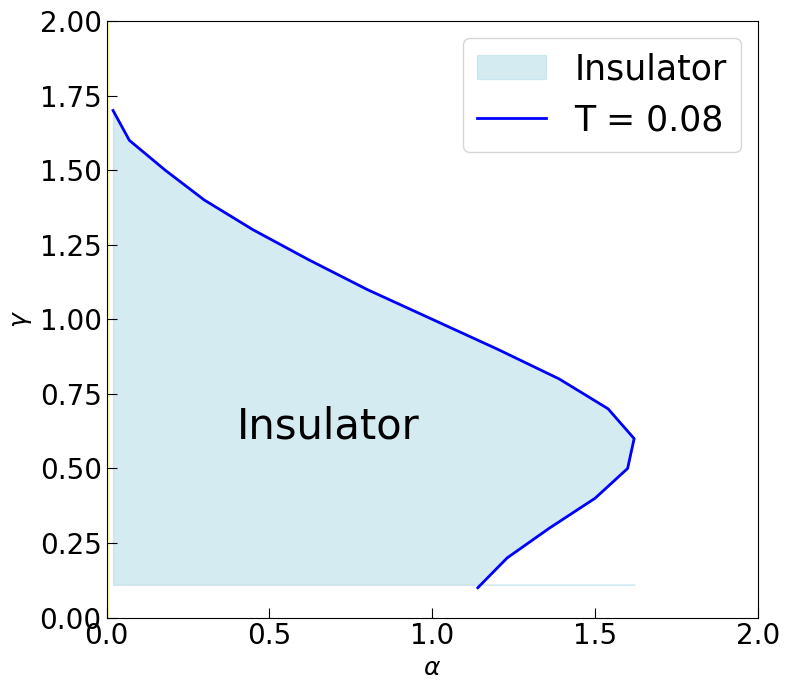
\includegraphics[width=7.5cm]{TexFigure/4/4_3_07_Simplefig.png}}
  \caption{Crossover tendency in $\alpha$ - $\gamma$ plane.}
\end{figure}
\pagebreak
\newpage
\begin{figure}[H]
  \centerline{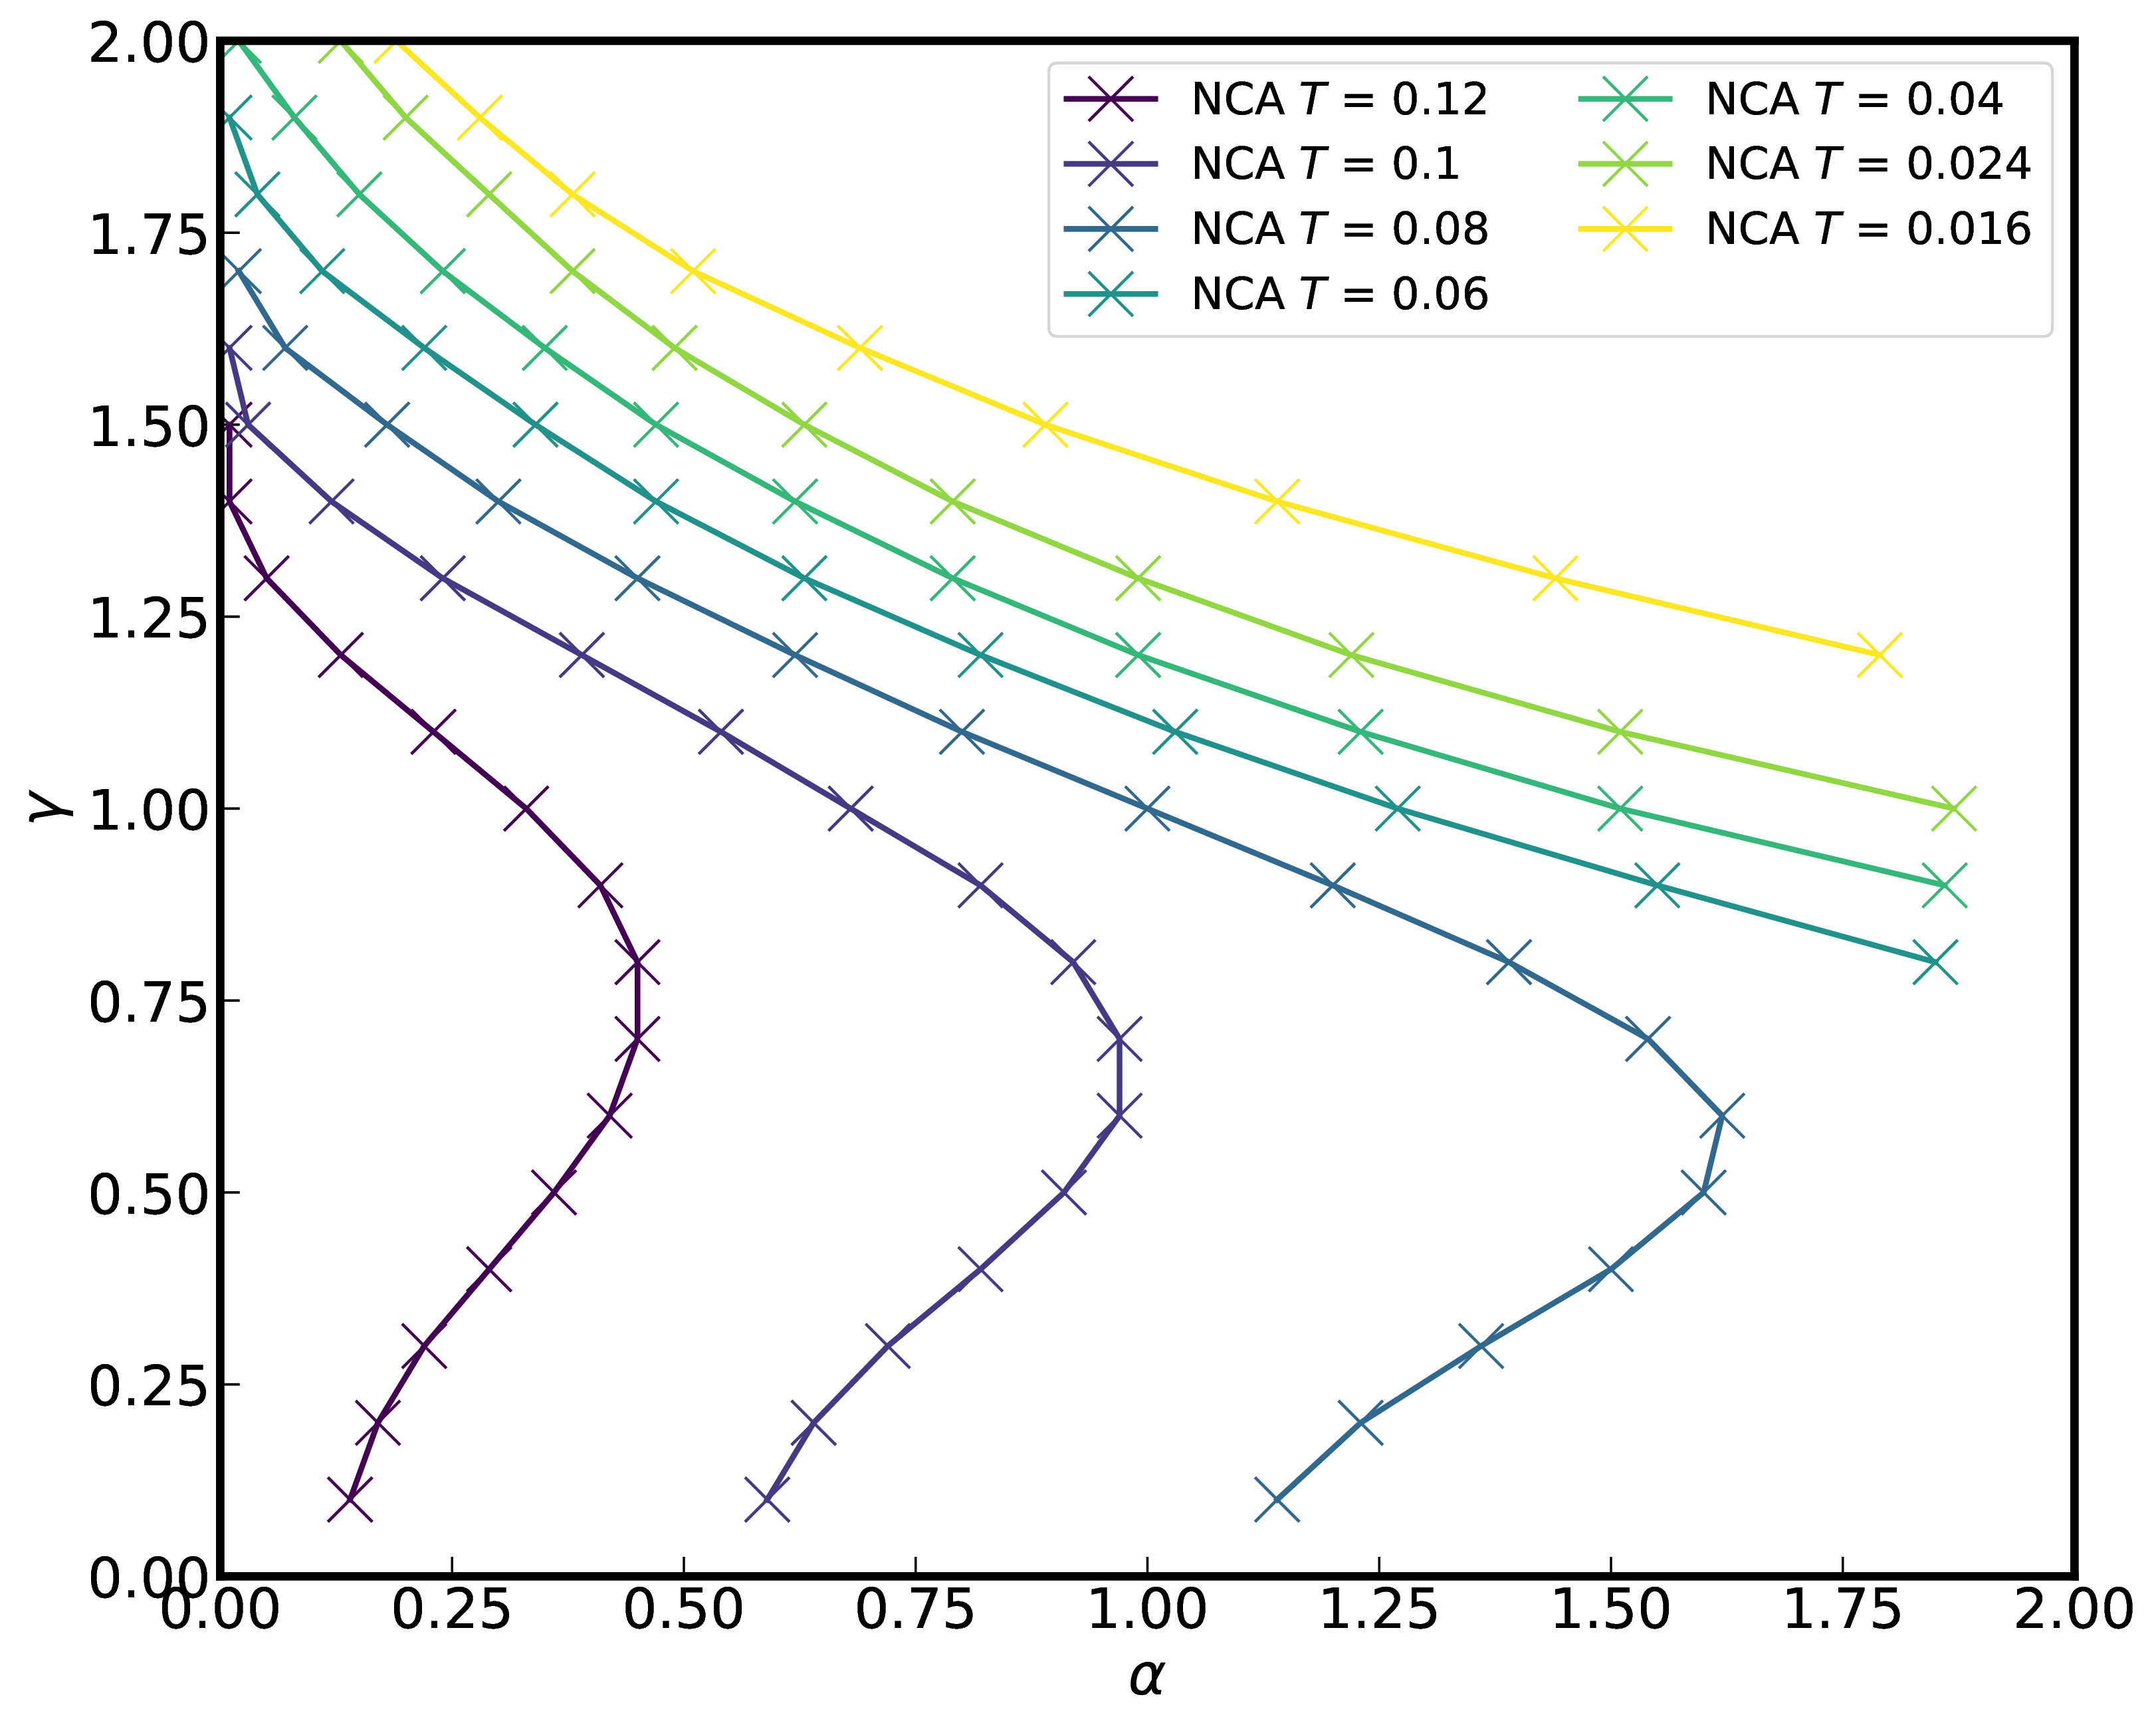
\includegraphics[width=13cm]{TexFigure/4/4_3_08_3dplot_Ns3_proj_n-1.png}}
  \centerline{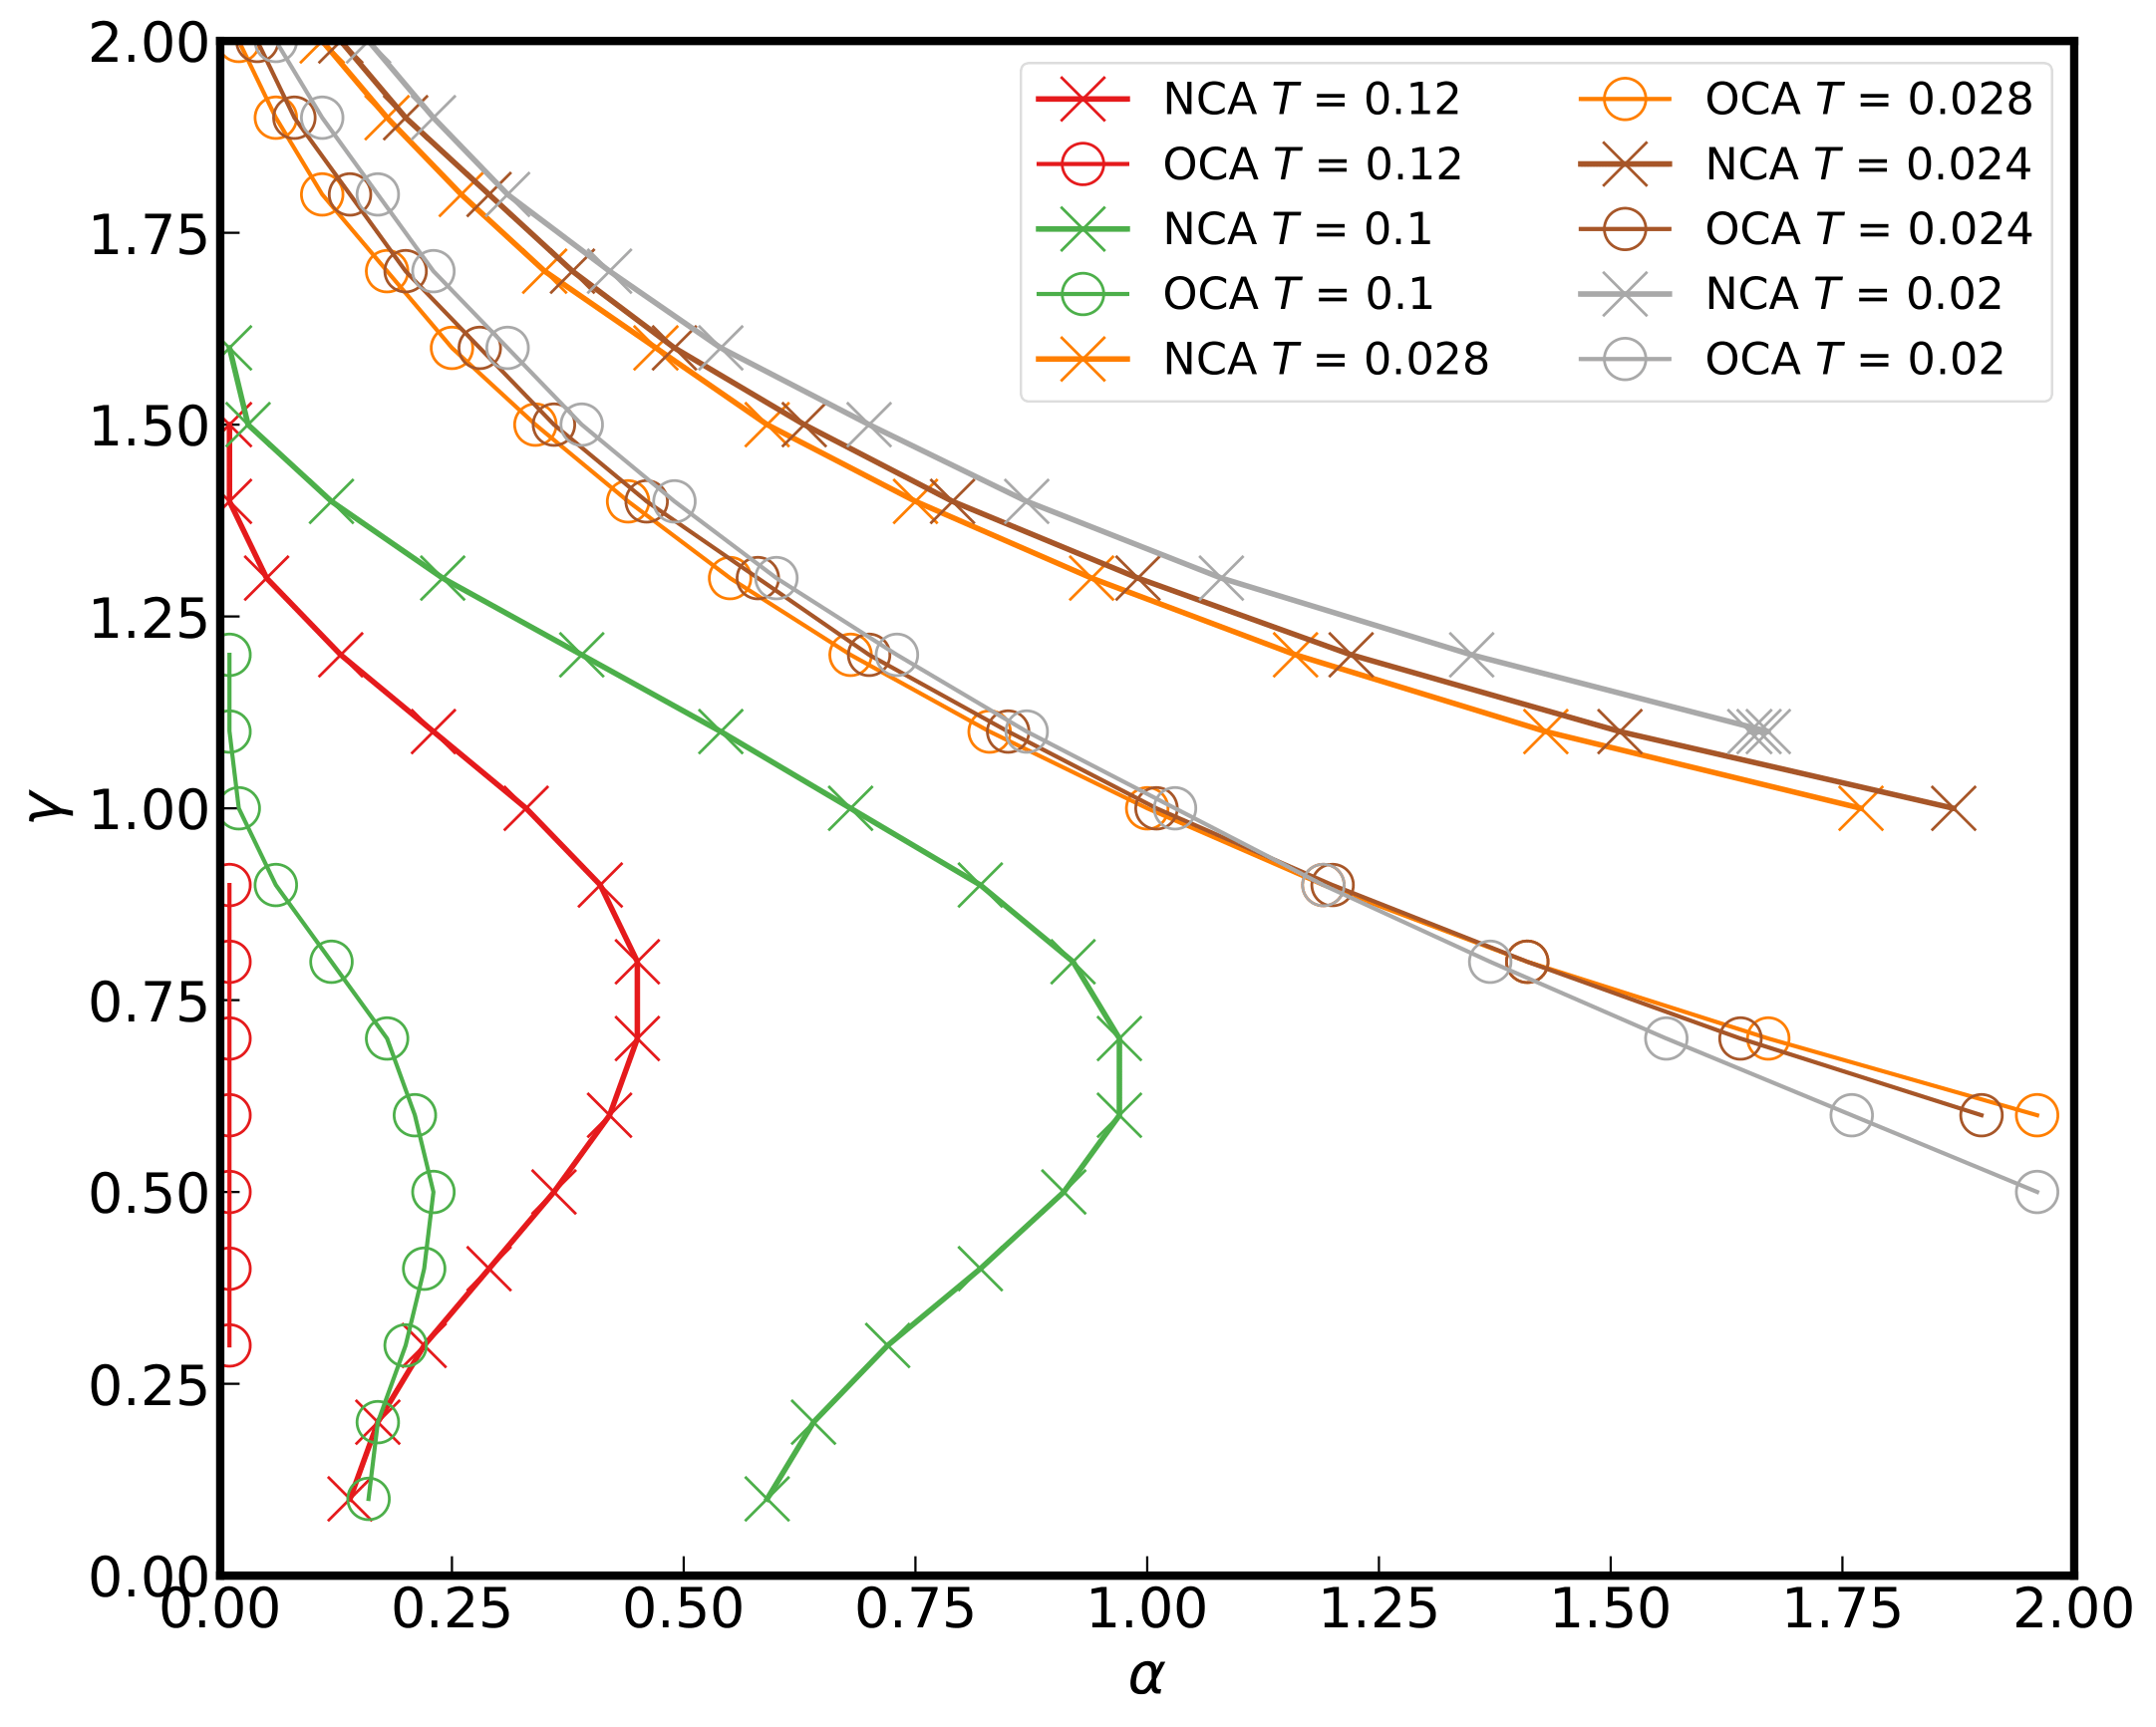
\includegraphics[width=13cm]{TexFigure/4/4_3_09_3dplot_COMP3_proj_n-1.png}}
  \caption{The points indicate where the sign change of the order parameter $\nu$ with temperature difference. Since differential was calculated in numerical method, noting that temperature is the lower value of the two discrete values 
  (e.g., T = 0.12 represents the line connecting the points where the $\nu$ values 
  difference for the two temperatures [0.1, 0.12] becomes 0). The upper plot shows the results calculated using NCA, 
  and the lower plot compares the results of OCA and NCA under the same temperature conditions.}
   \label{2Dplot}
\end{figure}
\begin{figure}[H]
  \centerline{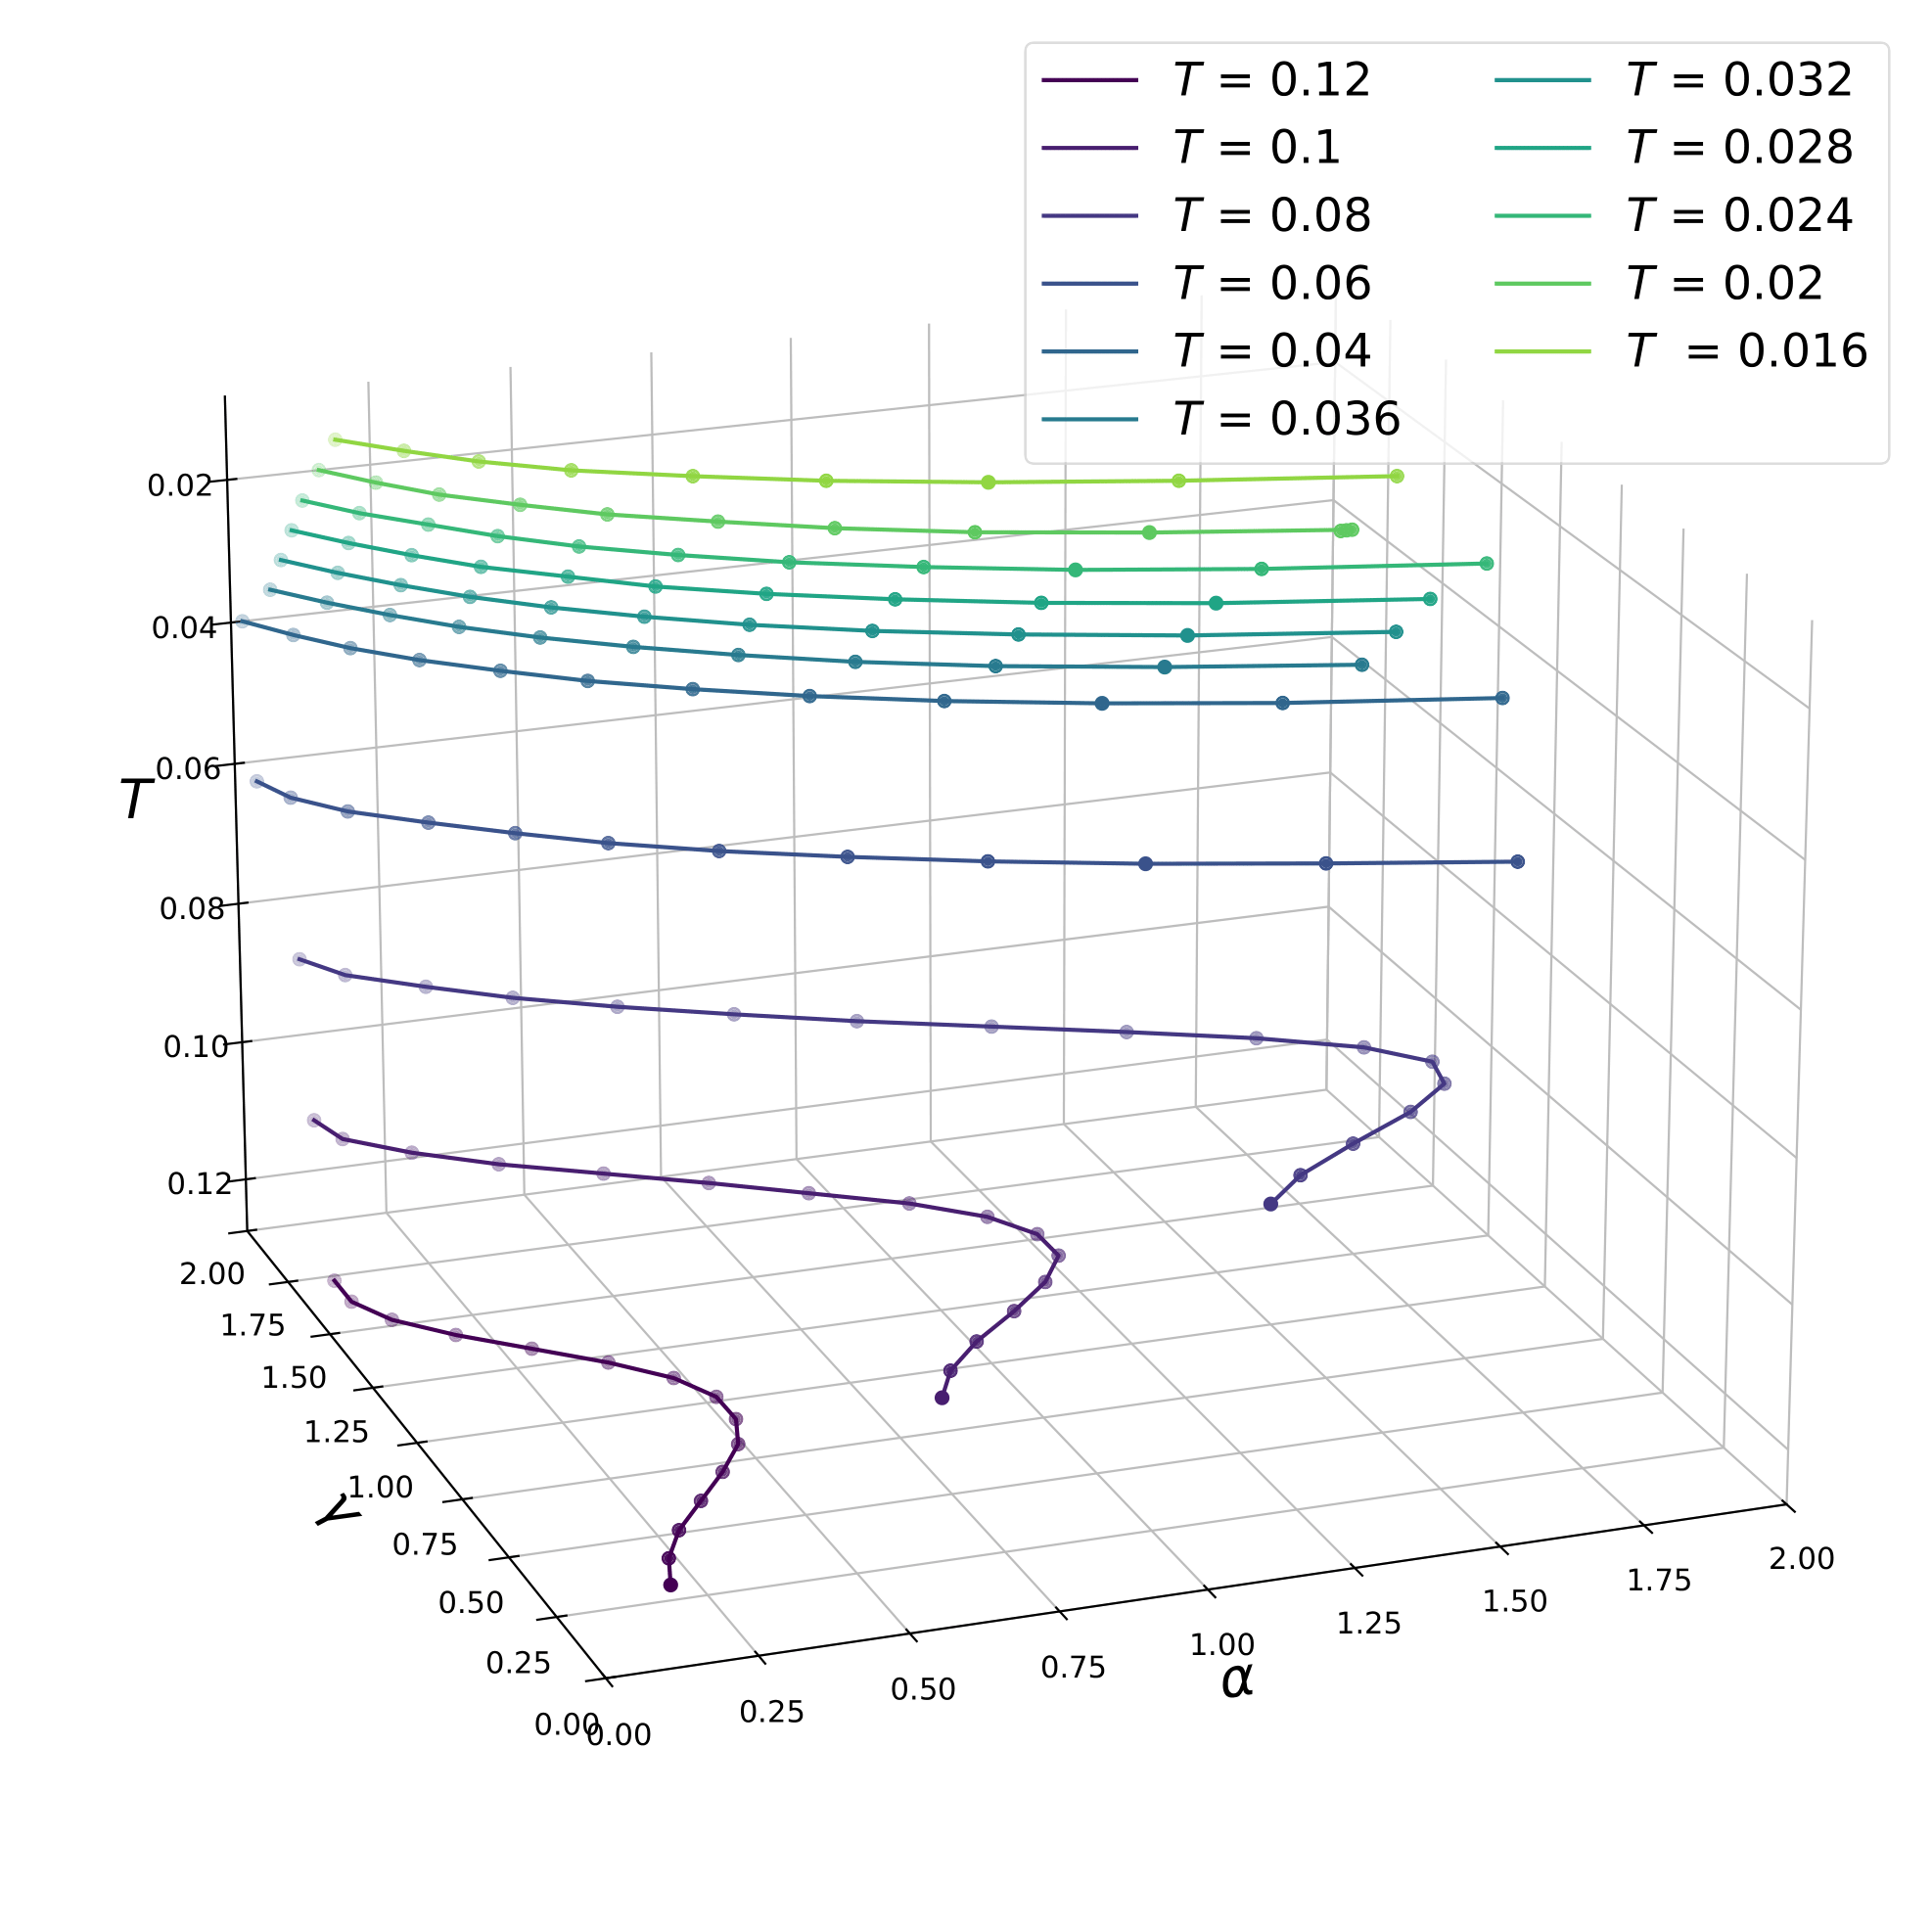
\includegraphics[width=13cm]{TexFigure/4/4_3_10_3dplot_Ns3_proj_20-1.png}}
  \caption{3-Dimension plotting of NCA result, with $T$ axis}%\ref{2Dplot}%,  with $\beta$ axis}
\end{figure}
\pagebreak
\begin{figure}[H]
  \vfill
  \centering
  \centerline{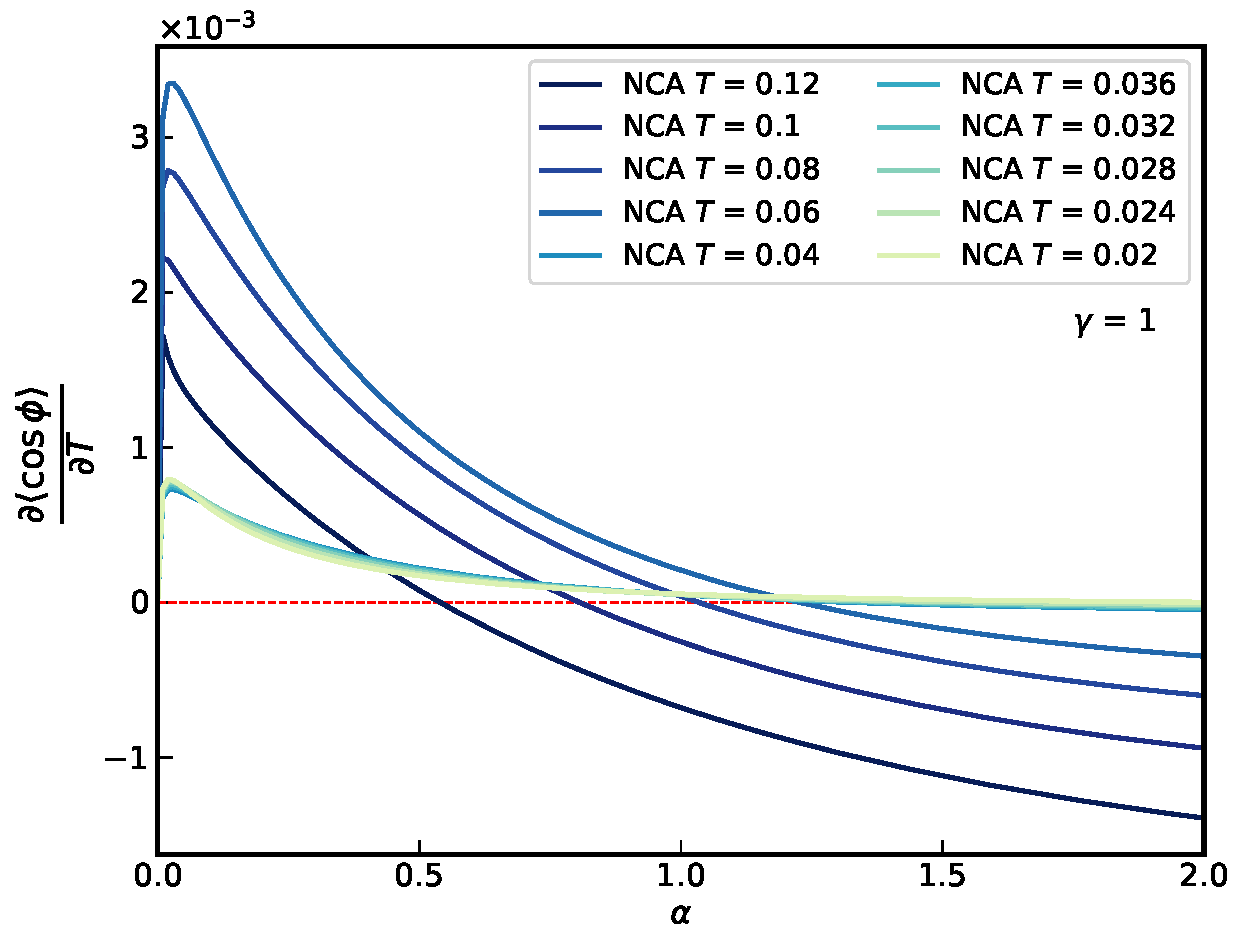
\includegraphics[width=9cm]{TexFigure/4/4_3_11_0.pdf}}
  \centerline{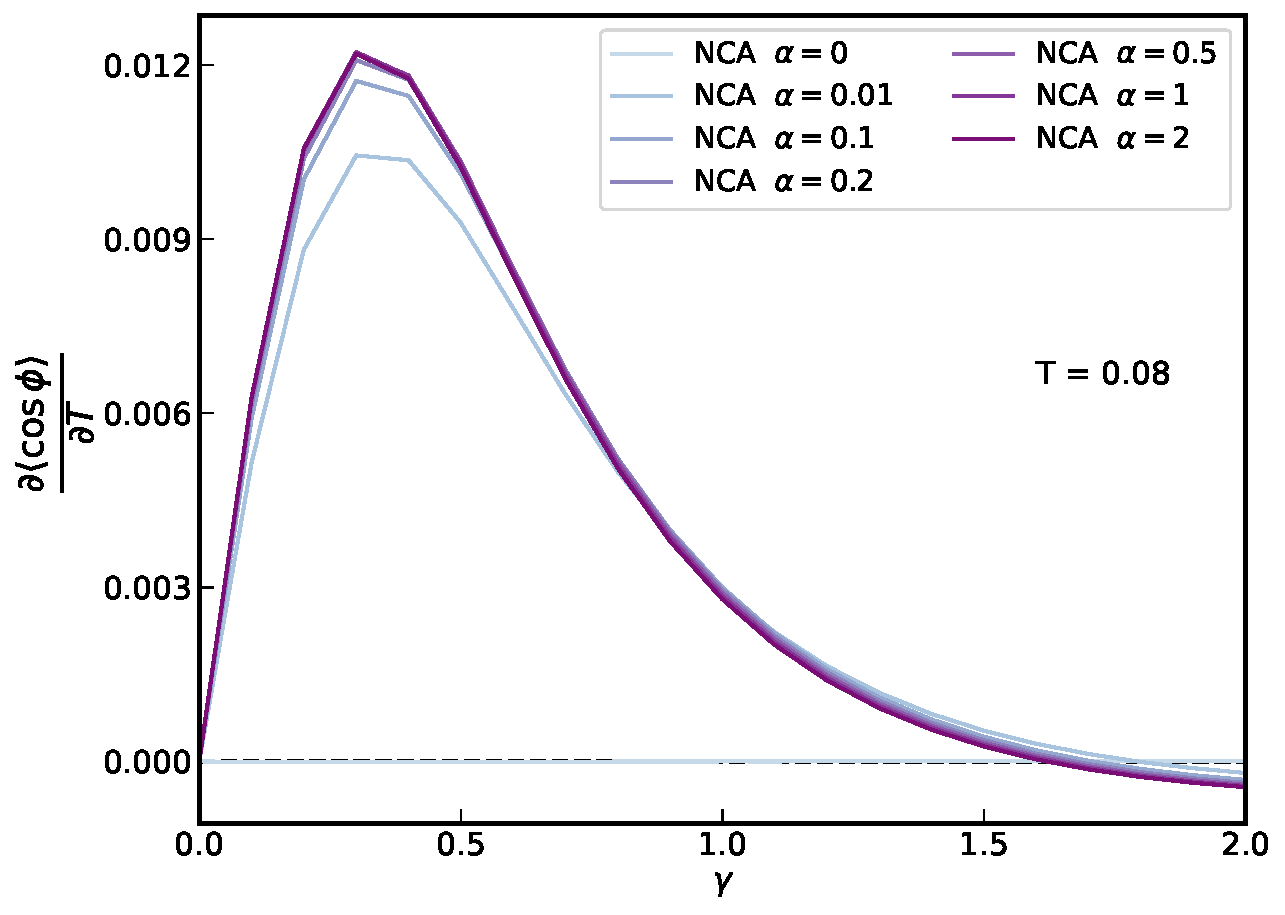
\includegraphics[width=9cm]{TexFigure/4/4_3_11_1.pdf}}
  \centerline{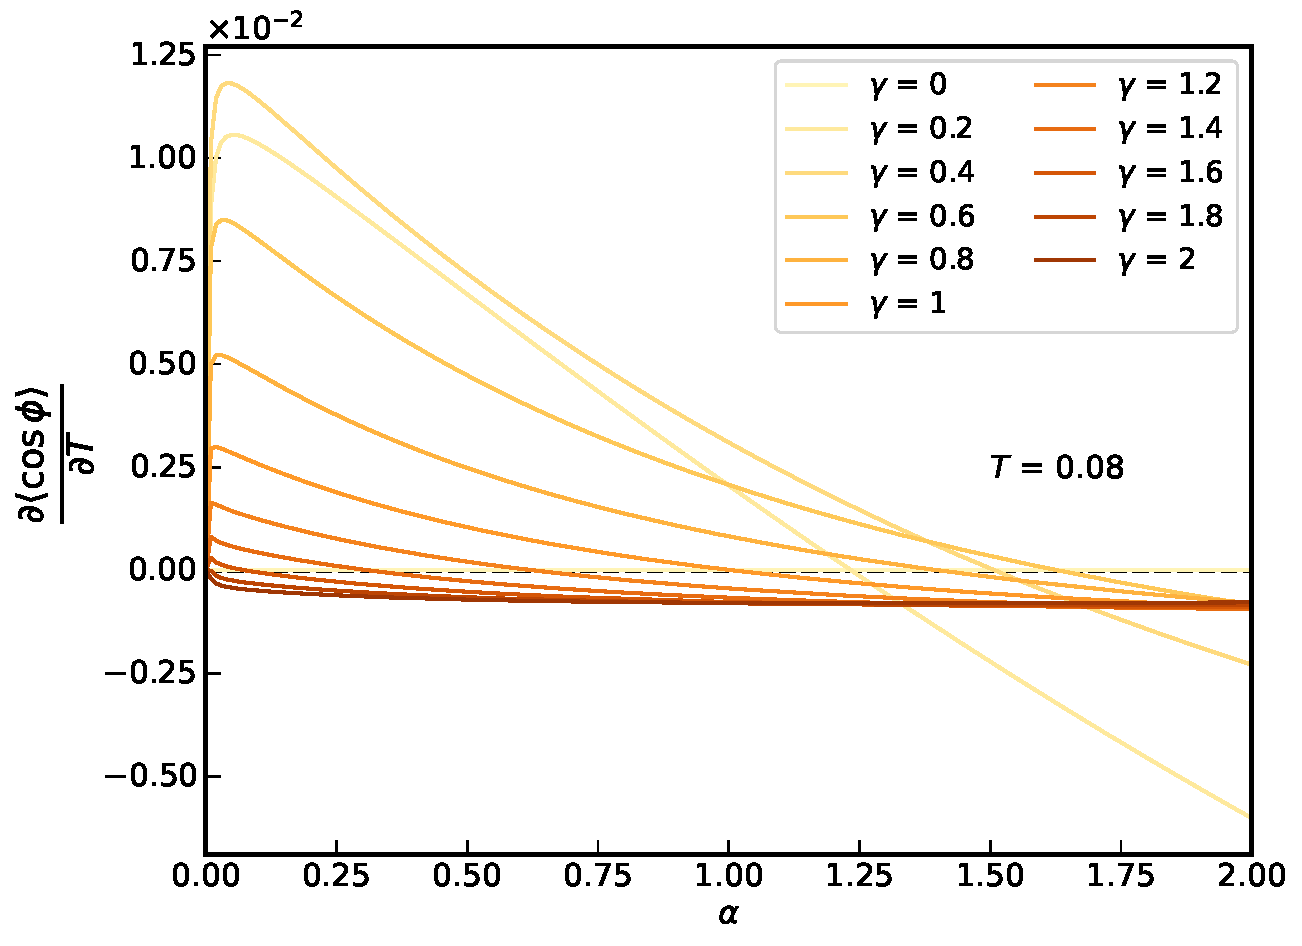
\includegraphics[width=9cm]{TexFigure/4/4_3_11_2.pdf}}
  \caption{Crossover tendency in a 2D plane corresponding to each pair of parameters. From upper, $\nu - \alpha$ plane over fixed $\gamma$ value, $\nu - \gamma$ over fixed $T$, $\nu-\alpha$ plane over fixed Temperature, respectively.}
  \vfill
\end{figure}
\pagebreak
\newpage
\subsubsection*{Small alpha}
In the calculation of $\hat{\cos\phi}$ at the value from $\alpha$ = 0 to near a small value, 
the system change shows a discontinuous behavior from superconductor to insulator. 
We can deduce two features:  \\
  \indent 1. when $\alpha=0$ there is no sign change in the order parameter,  \\
  \indent 2. The value of $\hat{\cos\phi}_{T_i}−\hat{\cos\phi}_{T_{i+1}}$ is always negative in $\alpha$ = 0, 
 suggesting that the system exhibits superconductivity. \\
 This contradicts the previous discussion that the left side of the crossover line should represent the insulator state. 
To investigate how the junction's phase change varies when the external environment's influence is small, 
we applied the approximation method in a small $\alpha$ interval. New alpha range follows:
\begin{table}[htbp]
  \centering
  \renewcommand{\arraystretch}{1.2}  % 행 간격 조정
  \begin{tabular}{@{}ccc@{}}
  \toprule
  \textbf{Previous $\alpha$} & \textbf{Updated $\alpha$} & \textbf{Interval}\\ 
  \midrule
  \text{[0,2]} & \text{[0,0.0001]} & 201 \\
  \bottomrule
  \end{tabular}
  \caption{Updated $\alpha$ range for simulation. Other conditions were left unchanged.}
  \end{table}
\begin{figure}[H]
  \centerline{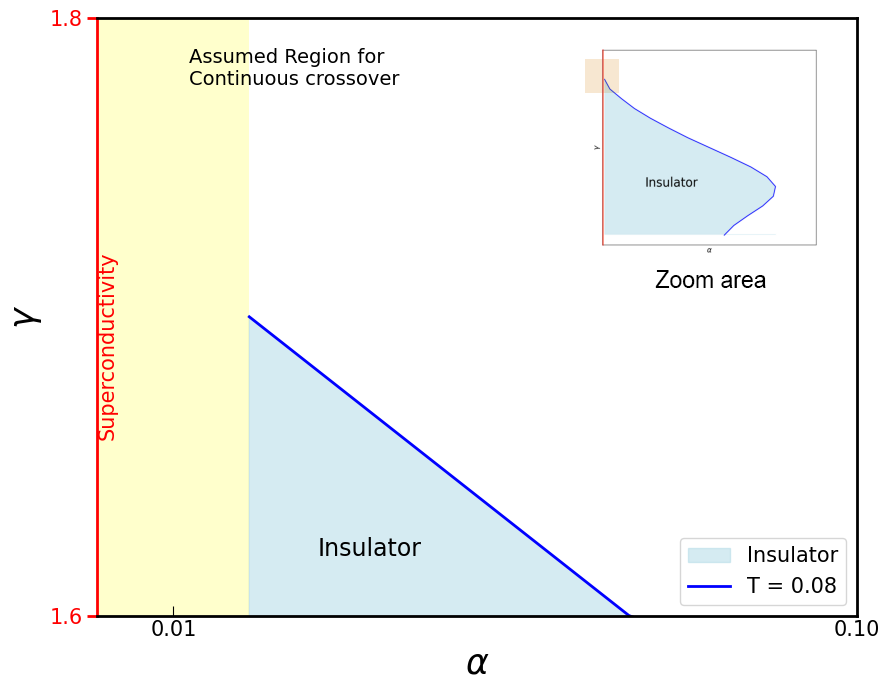
\includegraphics[width=7.5cm]{TexFigure/4/4_3_12_smallalp.png}}
  \caption{Expected temperature-dependent phase change behavior.
  the system will show continuity for its crossover tendency in the small $\alpha$ value interval.}
\end{figure}

The calculation results showed that the sign of $\frac{\partial \nu}{\partial T}$ changes from negative to positive 
as the $\gamma$ is varied within a specific temperature range. The existence of a continuous crossover from superconductor 
to insulator is presumed within a small $\alpha$ interval.
\pagebreak
\begin{figure}[H]
  \vfill
  \centerline{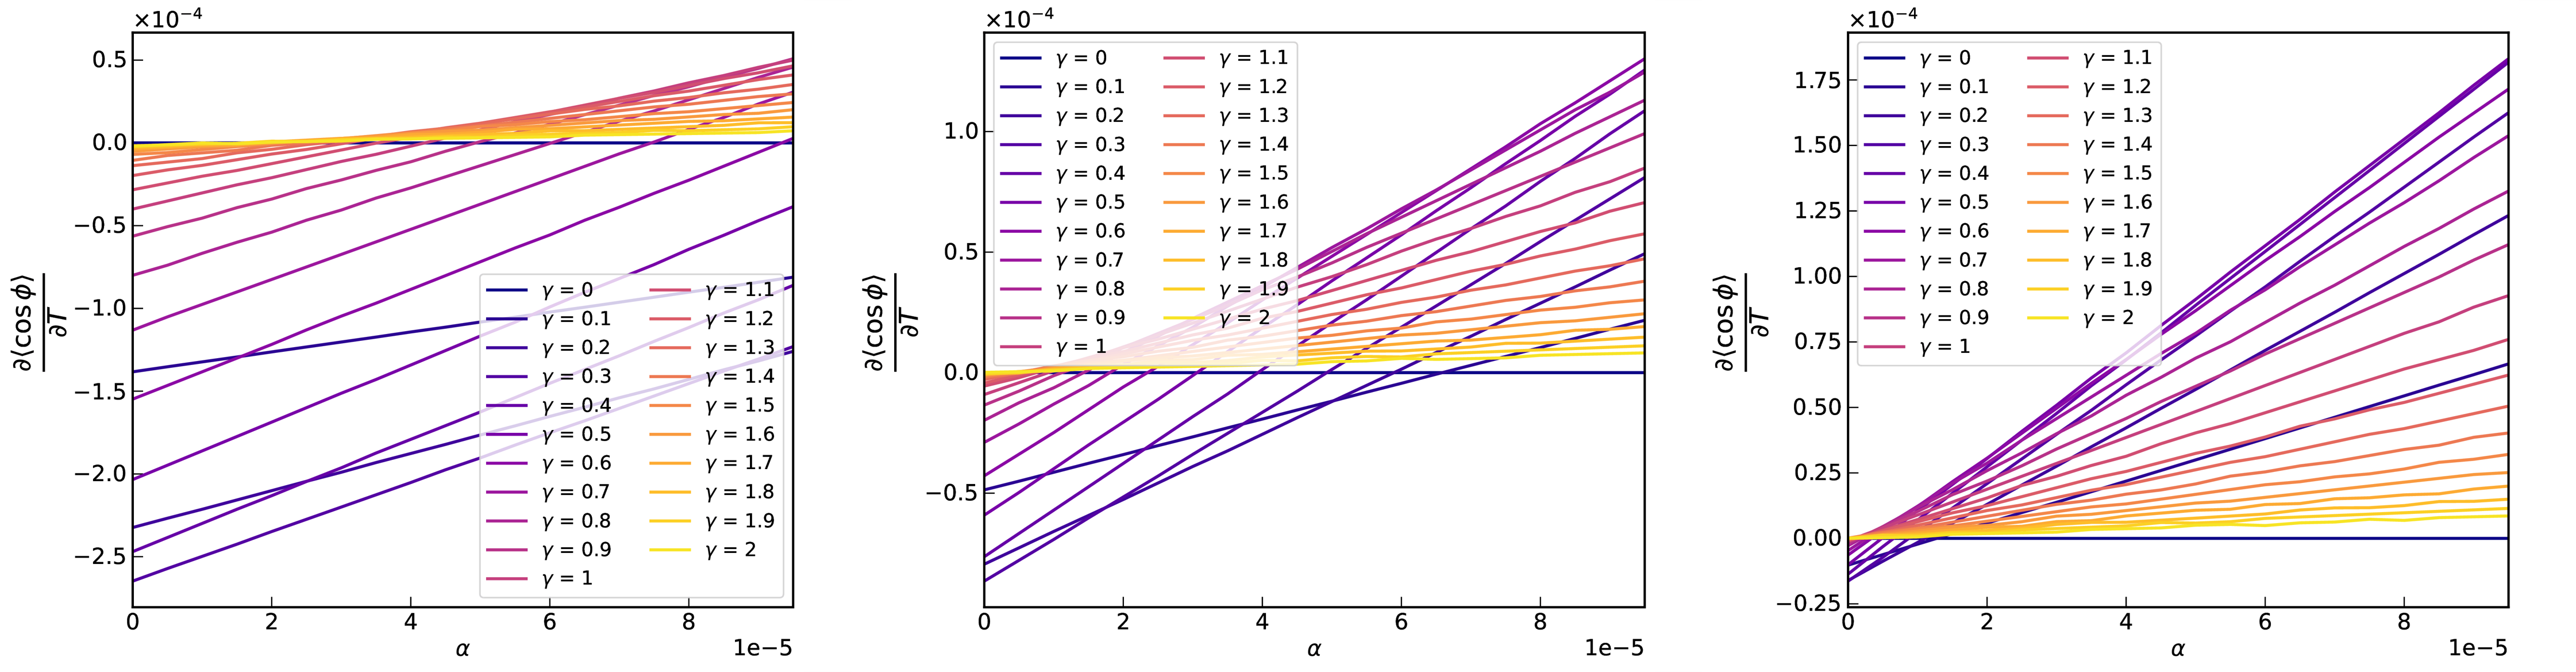
\includegraphics[width=15cm]{TexFigure/4/4_3_13_litlalp_1.png}}
  \caption{Crossover tendency calculated on NCA for fixed Temperature with varying $\gamma$ value in small $\alpha$ range. From the left, T = [0.14, 0.12], T = [0.12, 0.1], and T = [0.1, 0.08]. As the temperature decreases, the crossover behavior of $\frac{\partial \nu}{\partial T}$ 
  at large $\gamma$ values also decreases. This implies that at low temperatures, the crossover will not occur when the nonlinearity of the junction increases.}
  \vfill
\end{figure}
\begin{figure}[H]
  \centerline{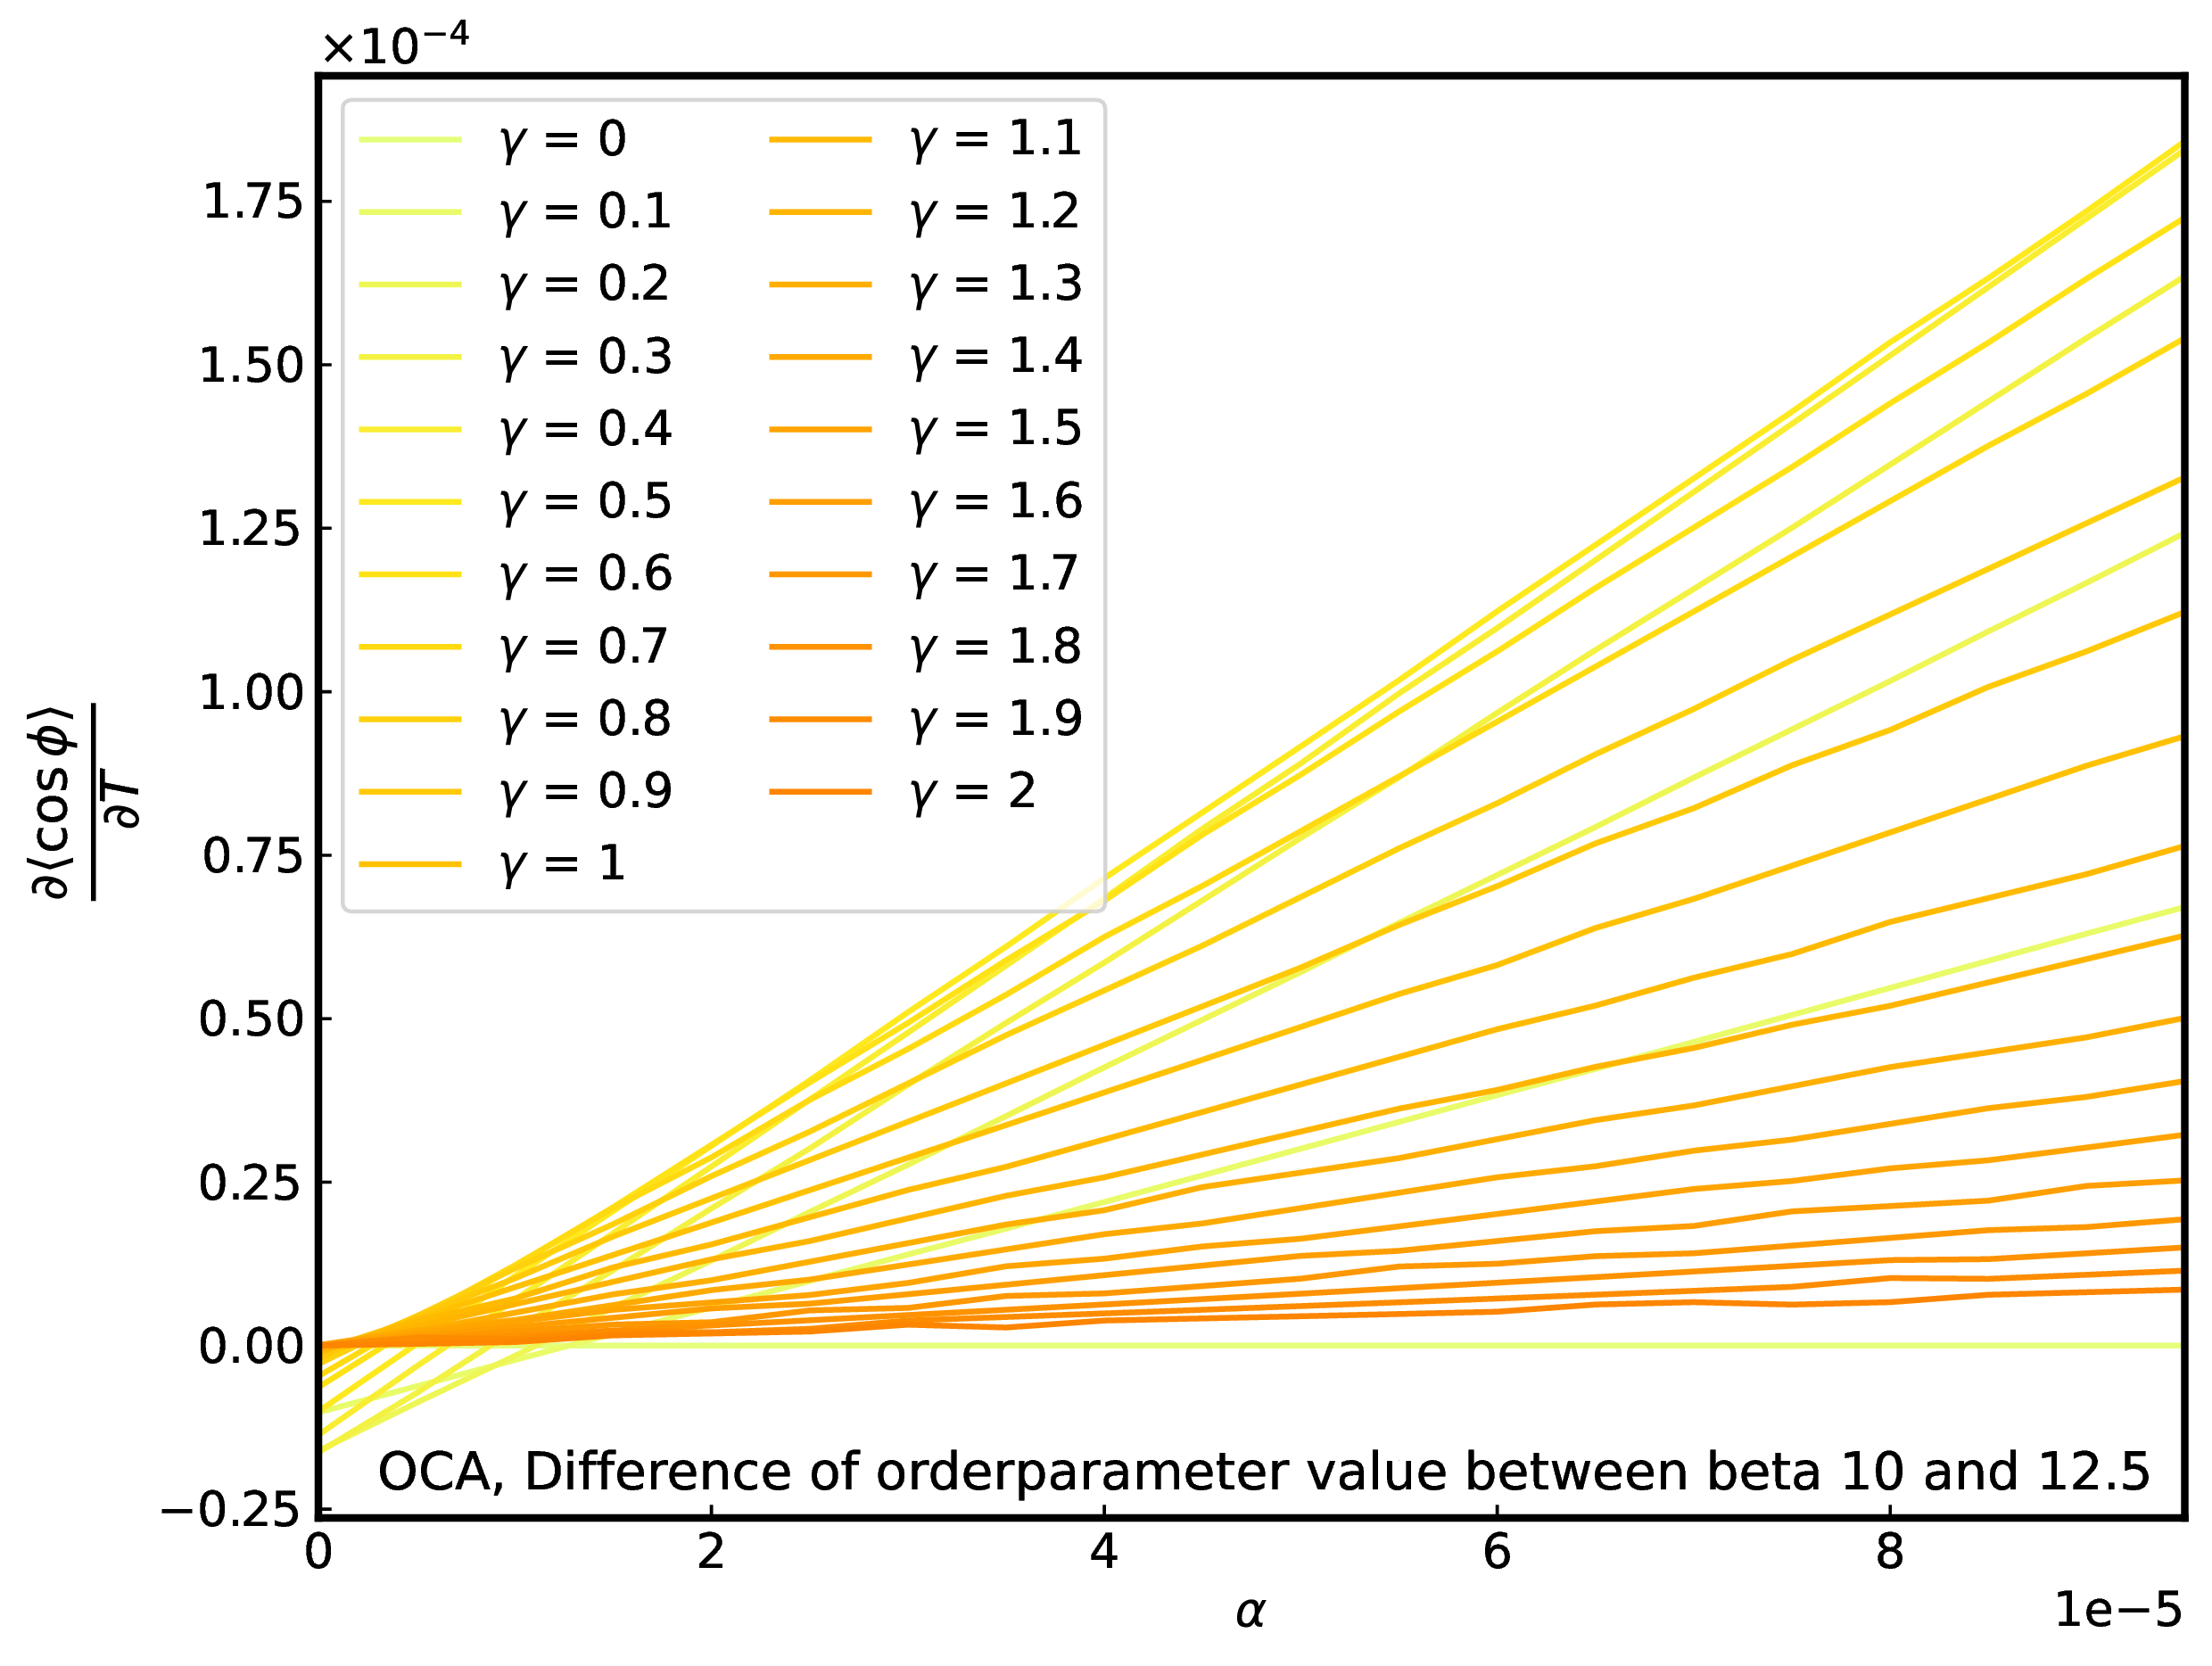
\includegraphics[width=9cm]{TexFigure/4/4_3_14_Diff_Os3_b_10_12.5_n.png}}
  \caption{Crossover tendency calculated on OCA. The temperature condition is T = [0.1,0.08].}
\vfill
\end{figure}
\pagebreak
\begin{figure}[H]
  \vfill
  \centerline{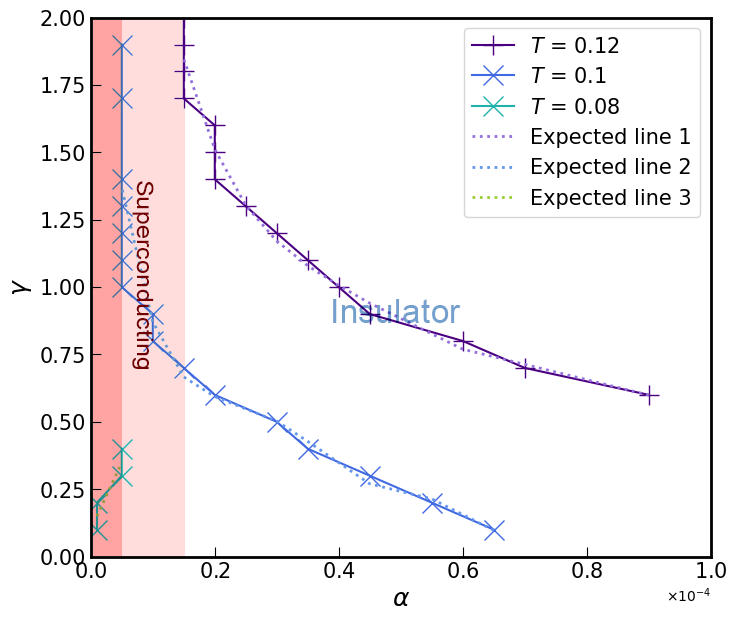
\includegraphics[width=13cm]{TexFigure/4/4_3_15_Expecregi.png}}
  \caption{Expected phase transition diagram. Expected crossover behavior is represented as a dotted line. 
   We can deduce as the temperature decreases, the insulator behavior becomes wider. }
  \vfill
  \end{figure}


\pagebreak
\newpage

\subsection{$\chi_{sp}$}
By calculating $\chi_{sp}(\tau)$ using the formula (2.59), we utilize the method of calculating approximation frequency, which has the formula:
\begin{flalign}
  \beta \chi_{sp}(\tau = \frac{\beta}{2})
\end{flalign}
\subsubsection*{Table. 4 condition}
We observed the following results: Varying the $\gamma$ value at a fixed $\alpha$ value, 
approximated value shows decreasing until $T = 0.1$ and towards to increase to decrease under $T=0.08$. 
When we fixed the $\gamma$ value and varied the $\alpha$ value, it increased in high temperatures but
decreased in low temperature as the $\alpha$ value increased.

\begin{figure}[H]
  \centerline{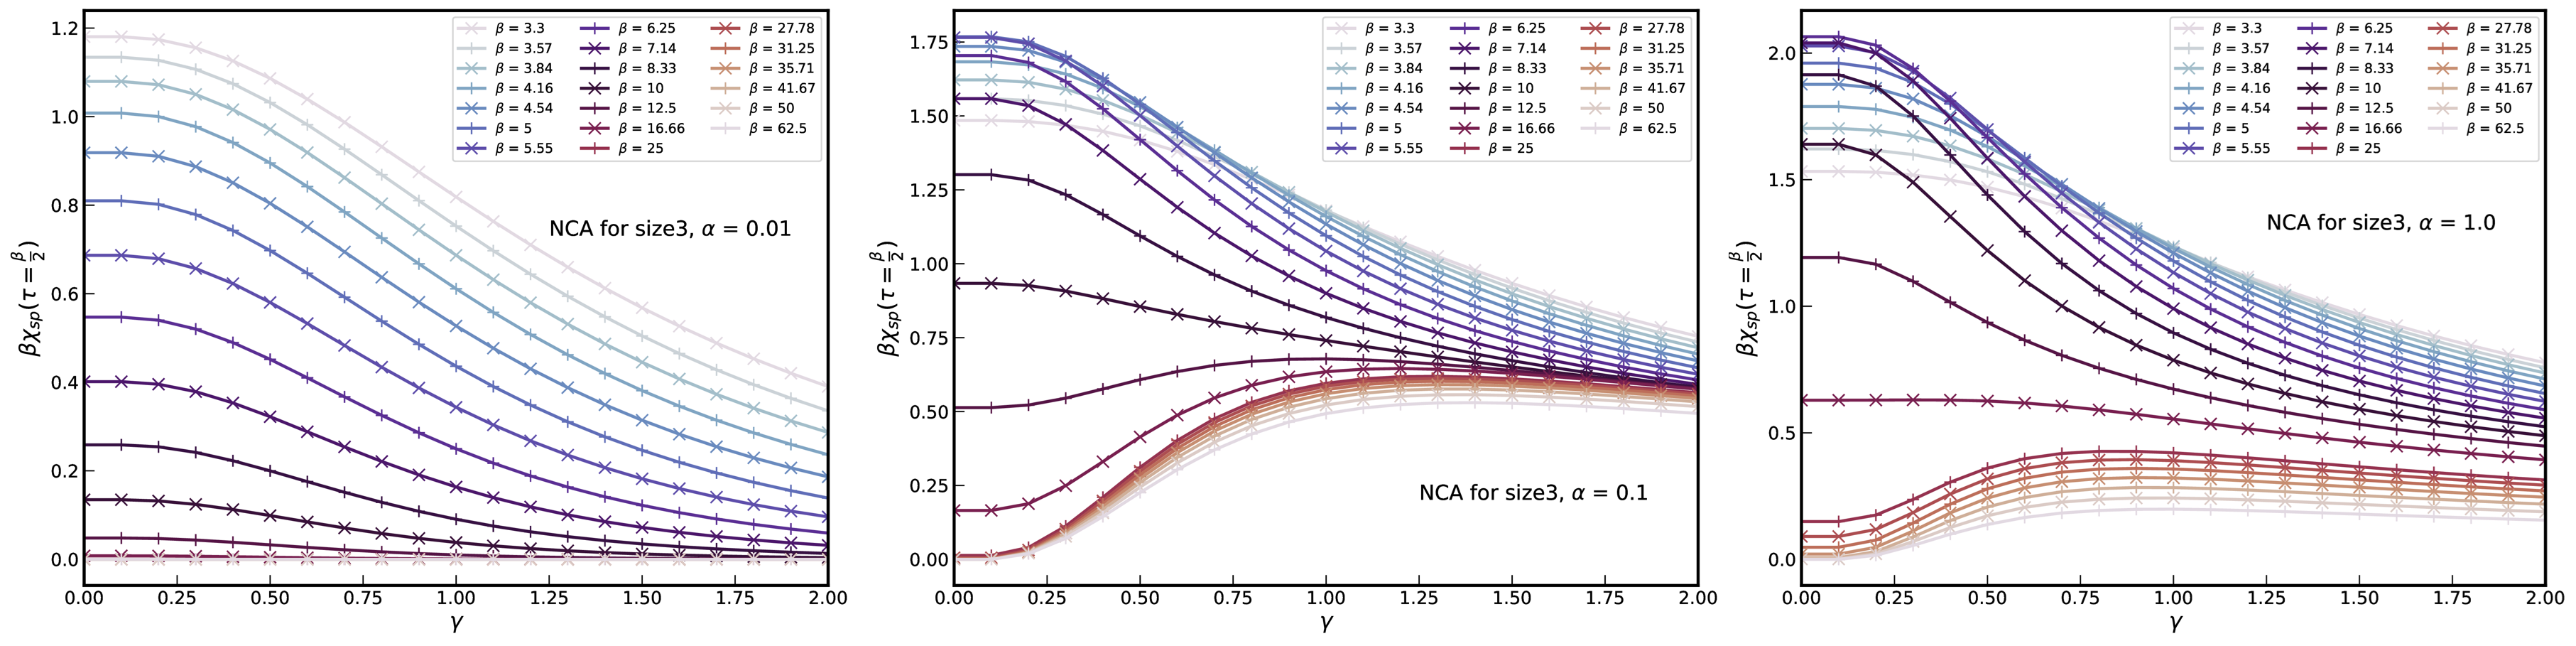
\includegraphics[width=15cm]{TexFigure/4/4_4_01_chi_gam_swp.png}}
  \centerline{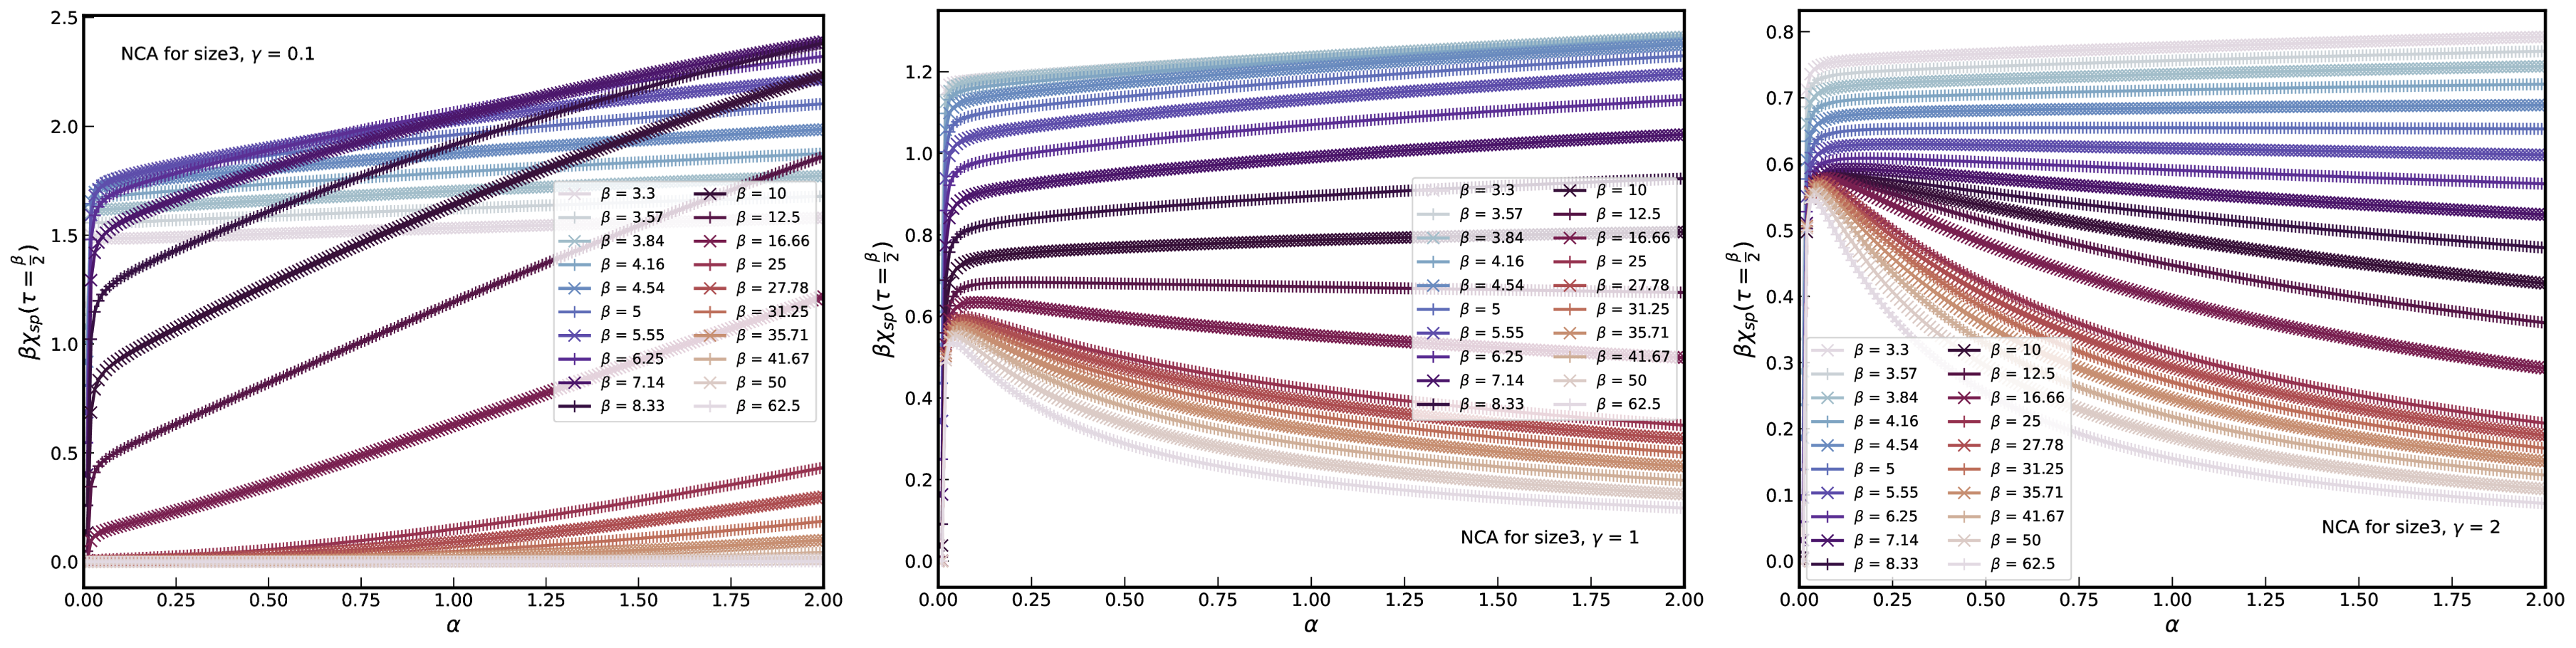
\includegraphics[width=15cm]{TexFigure/4/4_4_02_chi_alp_swp.png}}
  \caption{The crossing picture in $\chi_{sp}$ with $\gamma$ swapping and $\alpha$ swapping}
\end{figure}
\pagebreak
To observe how the phase changes for all $\gamma$ and $\alpha$ value conditions at a fixed temperature, 
we visualized the results using a 2D color map.  
We observed that the phase increased at high temperatures as the $\gamma$ and $\alpha$ values increased. 
At low temperatures, the phase generally decreased as the influence of the external environment increased. 
Yet the junction energy increased, and the phase tended to increase in more decisive influence from $\alpha$.
\begin{figure}[H]
  \centerline{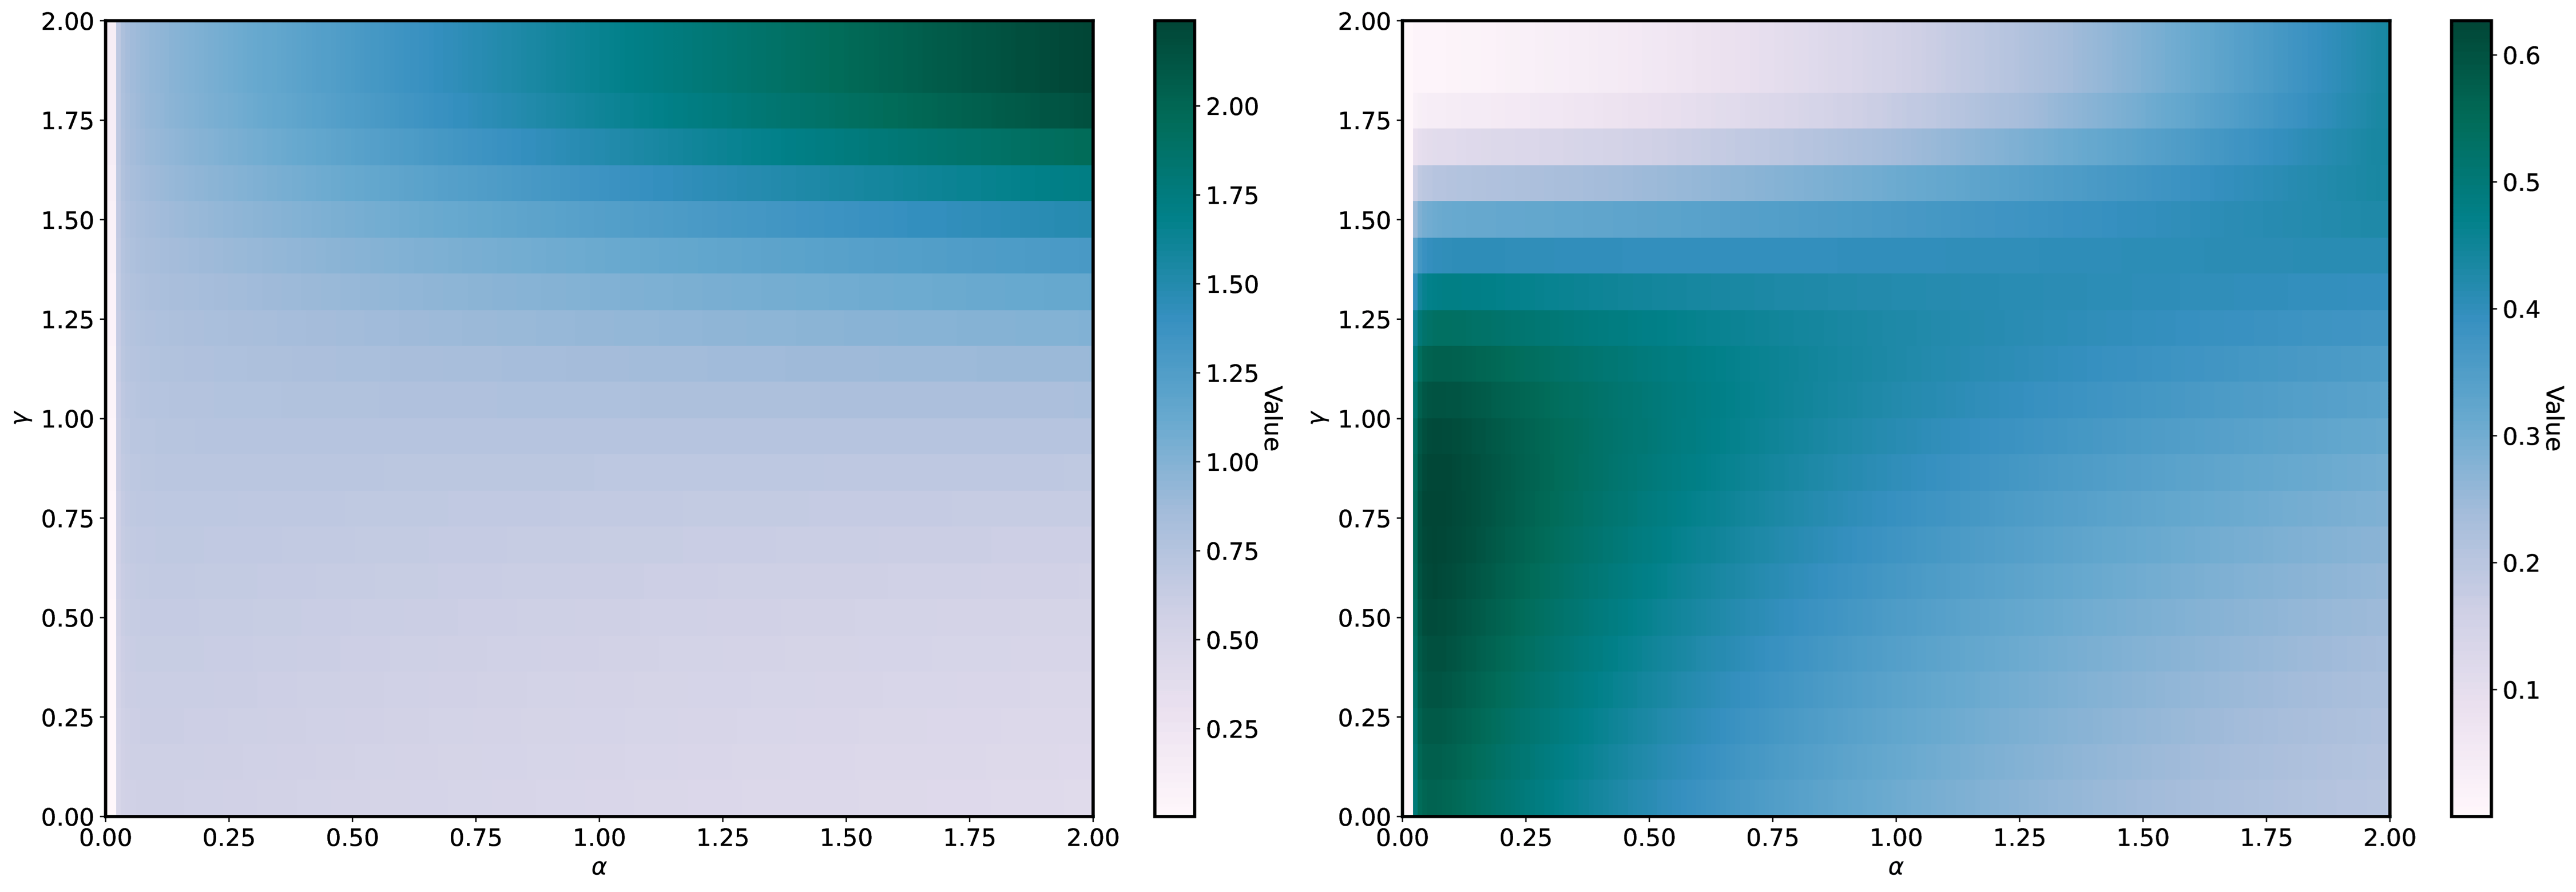
\includegraphics[width=13cm]{TexFigure/4/4_4_03_chi_color.png}}
  \caption{Colored plot for real frequency approximation. The simulation was performed in NCA. The left figure is for $\beta=10$; the Right is for $\beta=25$.
  The Josephson junction has high conductivity as the color goes deeper.}
 \end{figure}
\pagebreak
\subsubsection*{Exceeded $\alpha$ range}
In the crossover calculation using the approximation method using the correlation function, 
plotting the temperature-dependent behavior calculated with the approximation formula varying the influencing variables, 
the point where the lines corresponding to two consecutive temperatures intersect can be predicted as the crossover point.
The temperature-dependent phase approximation behavior was not observed within the previous set simulation range, 
we conducted calculations with a broader range of $\alpha$ values while maintaining the range of $\gamma$. 
It must be emphasized that the size of the $\tau$ grid was reduced for faster calculation verification. 
The range conditions used are shown in the table below.
\begin{table}[htbp]
  \centering
  \renewcommand{\arraystretch}{1.2}  % 행 간격 조정
  \begin{tabular}{@{}cccc@{}}
  \toprule
  \textbf{Variables} & \textbf{Min} & \textbf{Max}  & \textbf{Interval}\\ 
  \midrule
  $\gamma$ & 0 & 2 & 0.01 \\
  $\alpha$ & 0 & 20 & 1 \\
  $\beta$ & 3.3 & 25 &  \\
  Temperature & 0.3 & 0.04 & 0.02 \\
  \bottomrule
  \end{tabular}
  \caption{Exceeded parameter condition used for $\chi_{sp}$ calculation.}
  \end{table}
\begin{table}[htbp]
  \centering
  \renewcommand{\arraystretch}{1.2}  % 행 간격 조정
  \begin{tabular}{@{}ccc@{}}
  \toprule
  \textbf{Number} & \textbf{Interval} & \textbf{Gridsize}\\ 
  \midrule
  $\tau$ grid & [0,$\beta$] & 700 \\
  k grid & [0,K = 30000] & 30000 \\
  \bottomrule
  \end{tabular}
  \caption{Adjusted grid condition used for $\chi_{sp}$ calculation}
  \end{table}
\\
When the calculation was performed by increasing the $\gamma$ value for a fixed $\alpha$ value, crossing points occurred according to temperature, 
and it was confirmed that the points obtained within the temperature interval converged to a specific line as the $\alpha$ value increased. 
Based on the result, we draw the expected locations of the crossover points from the results calculated by the approximation method. 
The change of $\gamma$ as a function of $\alpha$ was re-plotted using the intersection points above. 
The color of each line corresponds to a different $\beta$ value.
Throughout the result, we confirmed that the prediction of the crossover point through approximation was not possible 
in the previous calculation range because no intersection value appeared at $\alpha$ values less than two at low temperatures. 
Also, we confirmed that the crossover interval using approximation decreased as the temperature decreased.
\pagebreak
\begin{figure}[H]
  \vfill
  \centerline{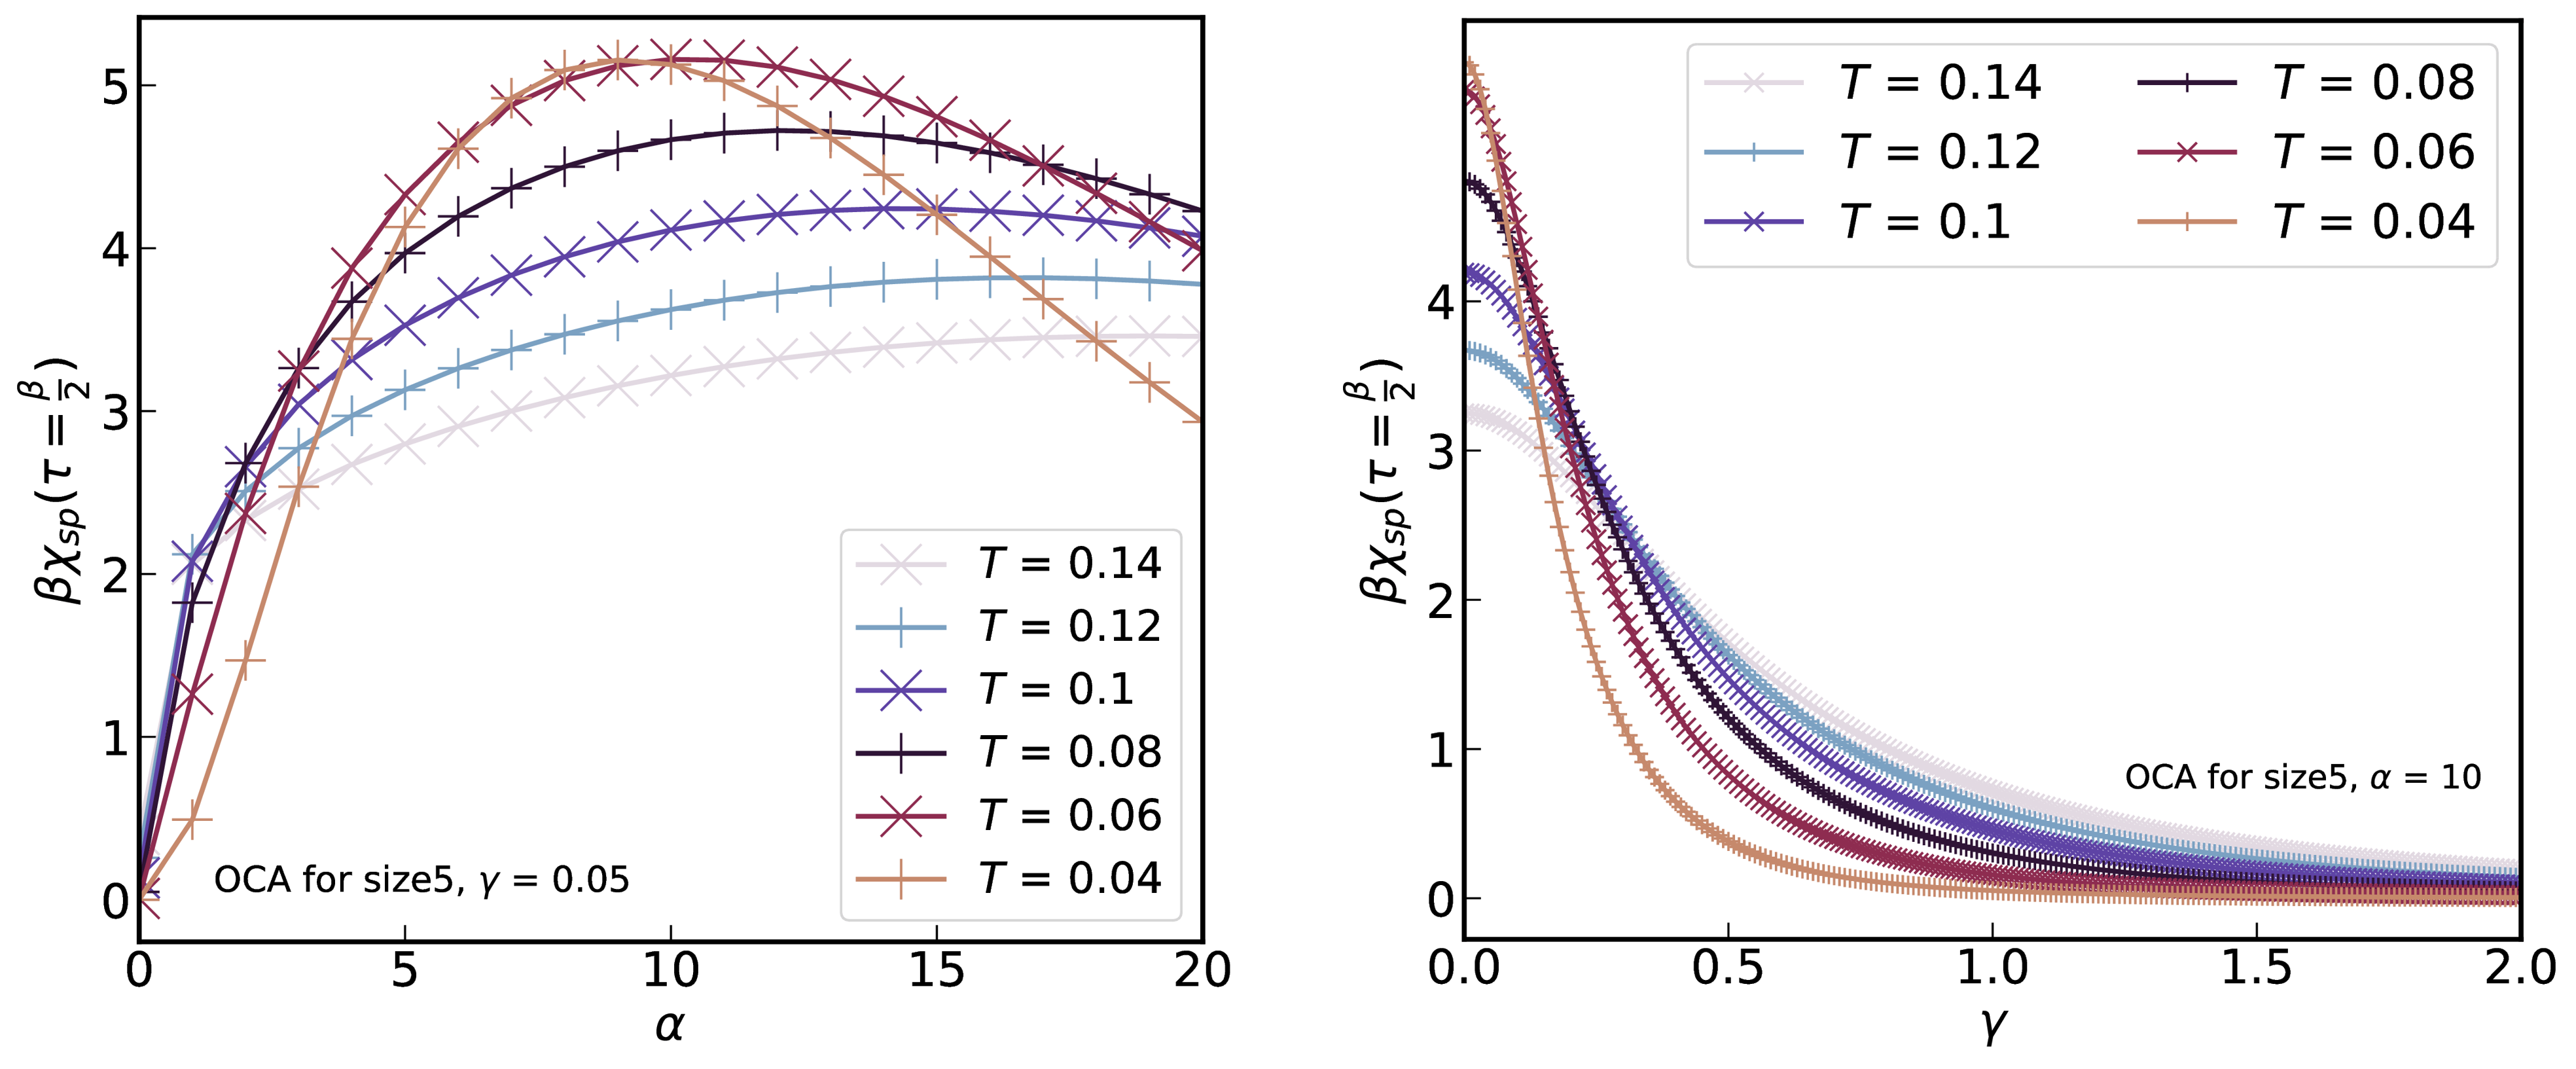
\includegraphics[width=13cm]{TexFigure/4/4_4_04_crossing.png}}
  \centerline{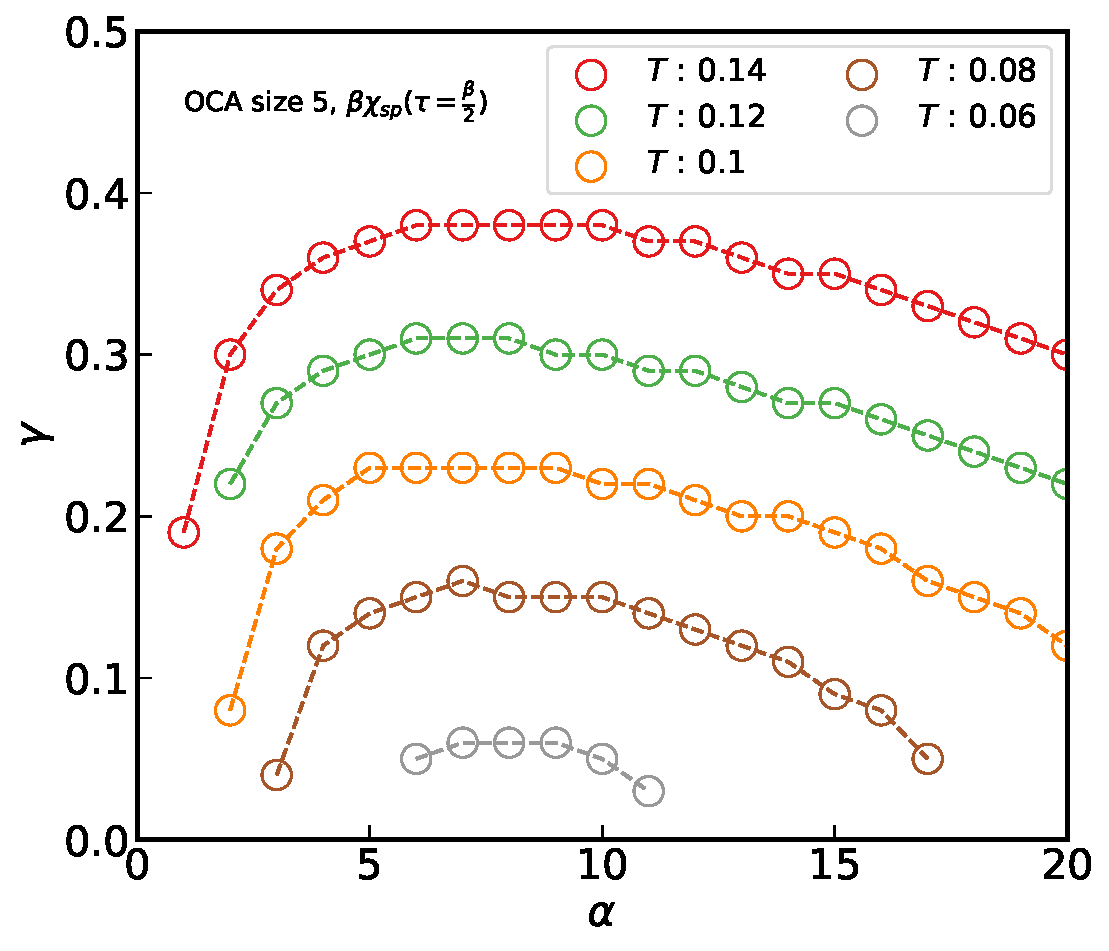
\includegraphics[width=13cm]{TexFigure/4/4_4_05_templine.pdf}}
  \caption{Crossover lines in extended $\alpha$ range. The below of the line is presumed to indicate that the system tends to insulate and the upper of the line is superconducting. The area of insulation decreases with temperature decreases.}
\vfill
\end{figure}
\pagebreak
\newpage
\begin{figure}[H]
  \centerline{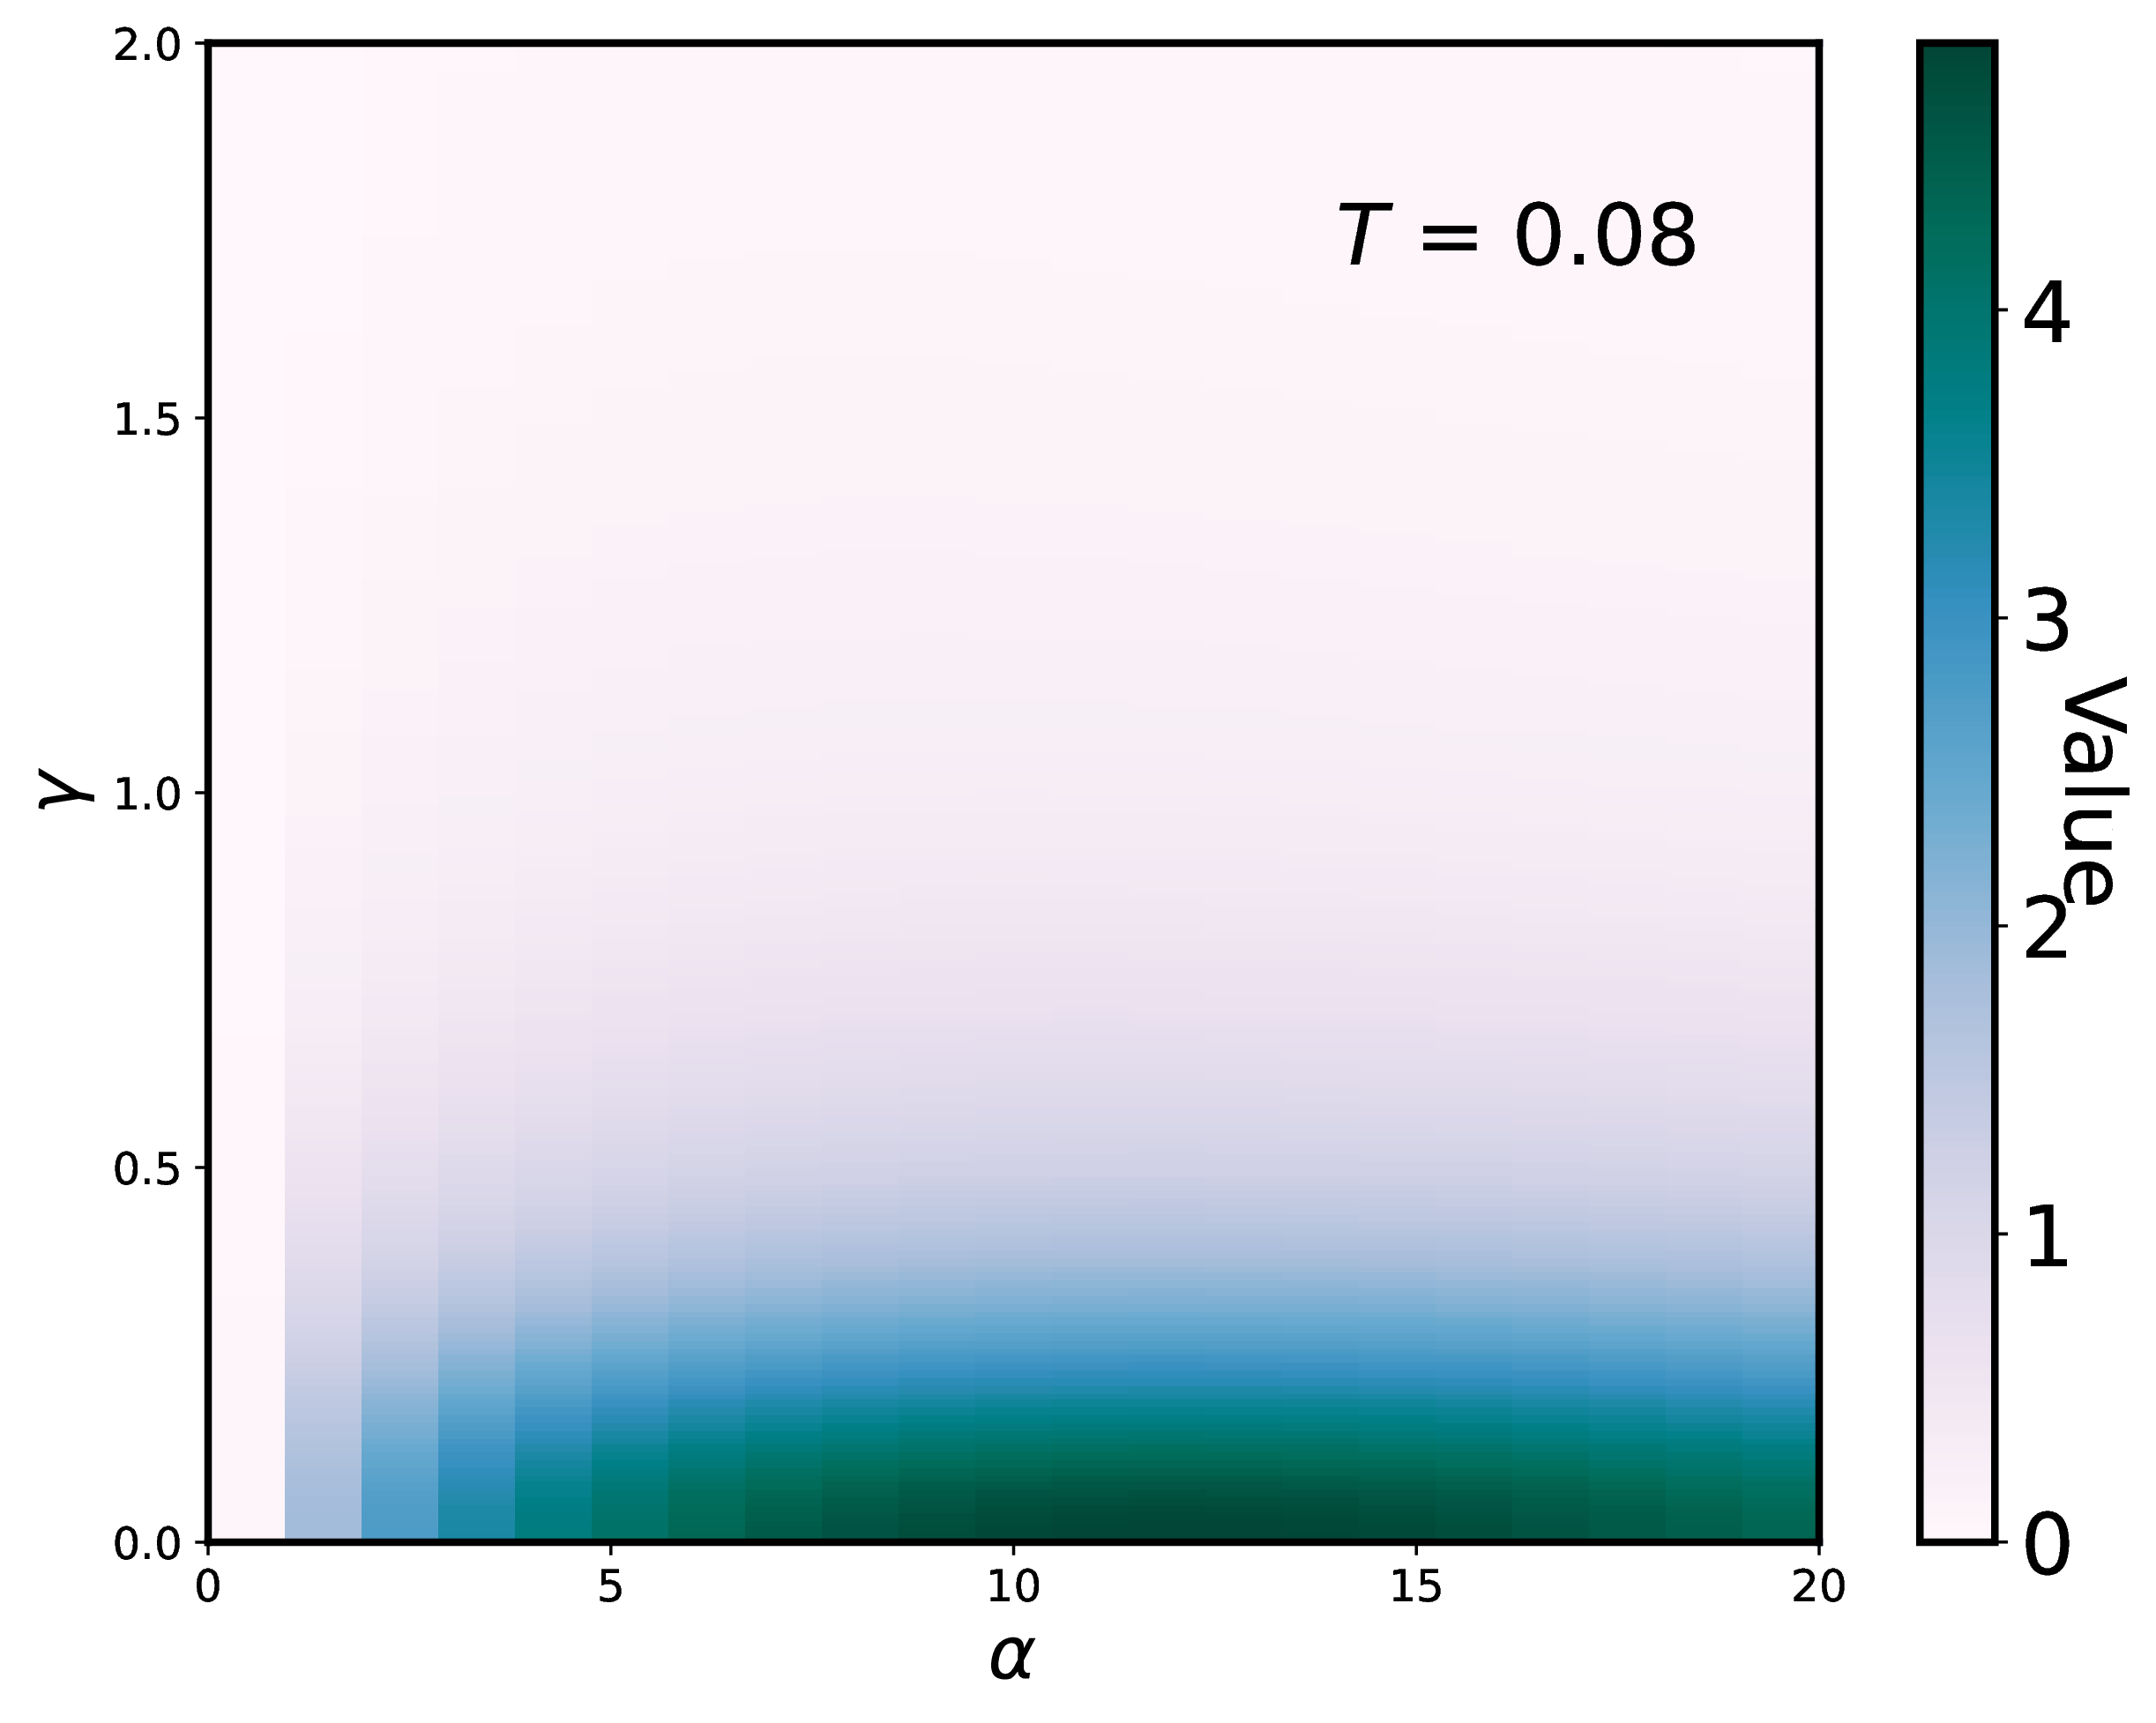
\includegraphics[width=9cm]{TexFigure/4/4_4_05_oc_colormap.png}}
  \caption{Colored plot for the $\chi_{sp}(\tau)$ in fixed Temperature T =0.08. The simulation was performed in OCA with truncated matrix size 5. Deeper color corresponds to a superconducting feature. Contradicts with the result from the order parameter calculation, the system presumed in superconductivity in low $\gamma$, with an extended $\alpha$ regime.}
 \end{figure}
\end{spacing}
\end{document}